\documentclass[a4paper, 14pt]{extarticle}
\usepackage[russian]{babel}
\usepackage[T1]{fontenc}
\usepackage{fontspec}
\usepackage{indentfirst}
\usepackage{enumitem}
\usepackage{graphicx}
\usepackage[
  left=20mm,
  right=10mm,
  top=20mm,
  bottom=20mm
]{geometry}
\usepackage{parskip}
\usepackage{titlesec}
\usepackage{xurl}
\usepackage{hyperref}
\usepackage{float}
\usepackage[
  figurename=Рисунок,
  labelsep=endash,
]{caption}
\usepackage[outputdir=build, newfloat]{minted}
\usepackage{multirow}
\usepackage{array}
\usepackage{tabularx}

\hypersetup{
  colorlinks=true,
  linkcolor=black,
  filecolor=blue,
  urlcolor=blue,
}

\renewcommand*{\labelitemi}{---}
\setmainfont{Times New Roman}
\setmonofont{JetBrains Mono}[
  SizeFeatures={Size=11},
]

\newenvironment{code}{\captionsetup{type=listing}}{}
\SetupFloatingEnvironment{listing}{name=Листинг}

\setminted{
  fontsize=\footnotesize,
  framesep=0mm,
}

\captionsetup{width=\textwidth,justification=centering}
\captionsetup[table]{singlelinecheck=off,justification=justified}

\newcolumntype{L}[1]{>{\raggedright\let\newline\\\arraybackslash\hspace{0pt}}m{#1}}
\newcolumntype{C}[1]{>{\centering\let\newline\\\arraybackslash\hspace{0pt}}m{#1}}
\newcolumntype{R}[1]{>{\raggedleft\let\newline\\\arraybackslash\hspace{0pt}}m{#1}}

\setlength{\parskip}{6pt}

\setlength{\parindent}{1cm}
\setlist[itemize]{itemsep=0em,topsep=0em,parsep=0em,partopsep=0em,leftmargin=2.0cm}
\setlist[enumerate]{itemsep=0em,topsep=0em,parsep=0em,partopsep=0em,leftmargin=2.0cm}

\renewcommand{\thesection}{\arabic{section}.}
\renewcommand{\thesubsection}{\thesection\arabic{subsection}.}
\renewcommand{\thesubsubsection}{\thesubsection\arabic{subsubsection}.}

\titleformat{\section}{\normalfont\bfseries}{\thesection}{0.5em}{}
\titleformat{\subsection}{\normalfont\bfseries}{\thesubsection}{0.5em}{}

\titleformat*{\section}{\normalfont\bfseries}
\titleformat*{\subsection}{\normalfont\bfseries}

\linespread{1.5}
\renewcommand{\baselinestretch}{1.5}
\begin{document}

\begin{titlepage}
  \vspace{0pt plus2fill}
  \noindent

  \vspace{0pt plus6fill}
  \begin{center}
    Санкт-Петербургский национальный исследовательский университет
    информационных технологий, механики и оптики

    \vspace{0pt plus2fill}

    Факультет инфокоммуникационных технологий

    Направление подготовки 11.03.02

    \vspace{0pt plus2fill}

    Практическая работа №5

    \vspace{0pt plus1fill}

    Изучение работы протоколов стека TCP/IP \\ с помощью Wireshark

  \end{center}

  \vspace{0pt plus7fill}
  \begin{flushright}
    Выполнил: \\
    Швалов Даниил Андреевич

    Группа: К33211

    Проверил: \\
    Харитонов Антон
  \end{flushright}

  \vspace{0pt plus2fill}
  \begin{center}
    Санкт-Петербург

    2023
  \end{center}
\end{titlepage}

\setcounter{page}{2}

\section{Введение}

\textbf{Цель работы}: разобраться со стеком TCP/IP, анализируя пакеты, которые
отправляются и принимаются с помощью данного стека, научиться собирать сетевой
трафик с помощью программы Wireshark, научиться фильтровать собранный трафик,
находить и просматривать соединения.

\section{Ход работы}

\subsection{Начало работы с Wireshark}

Для того, чтобы настроить перехват трафика на интерфейсе так, чтобы он
завершился после сбора 5 Мб, необходимо на панели нажать <<Capture>>, перейти в
<<Options>> и во вкладке <<Options>> в разделе <<Stop capture automatically
after>> указать <<5 megabytes>> (рис. \ref{fig:stop-capture-after-5-mb}).

\begin{figure}[H]
  \centering
  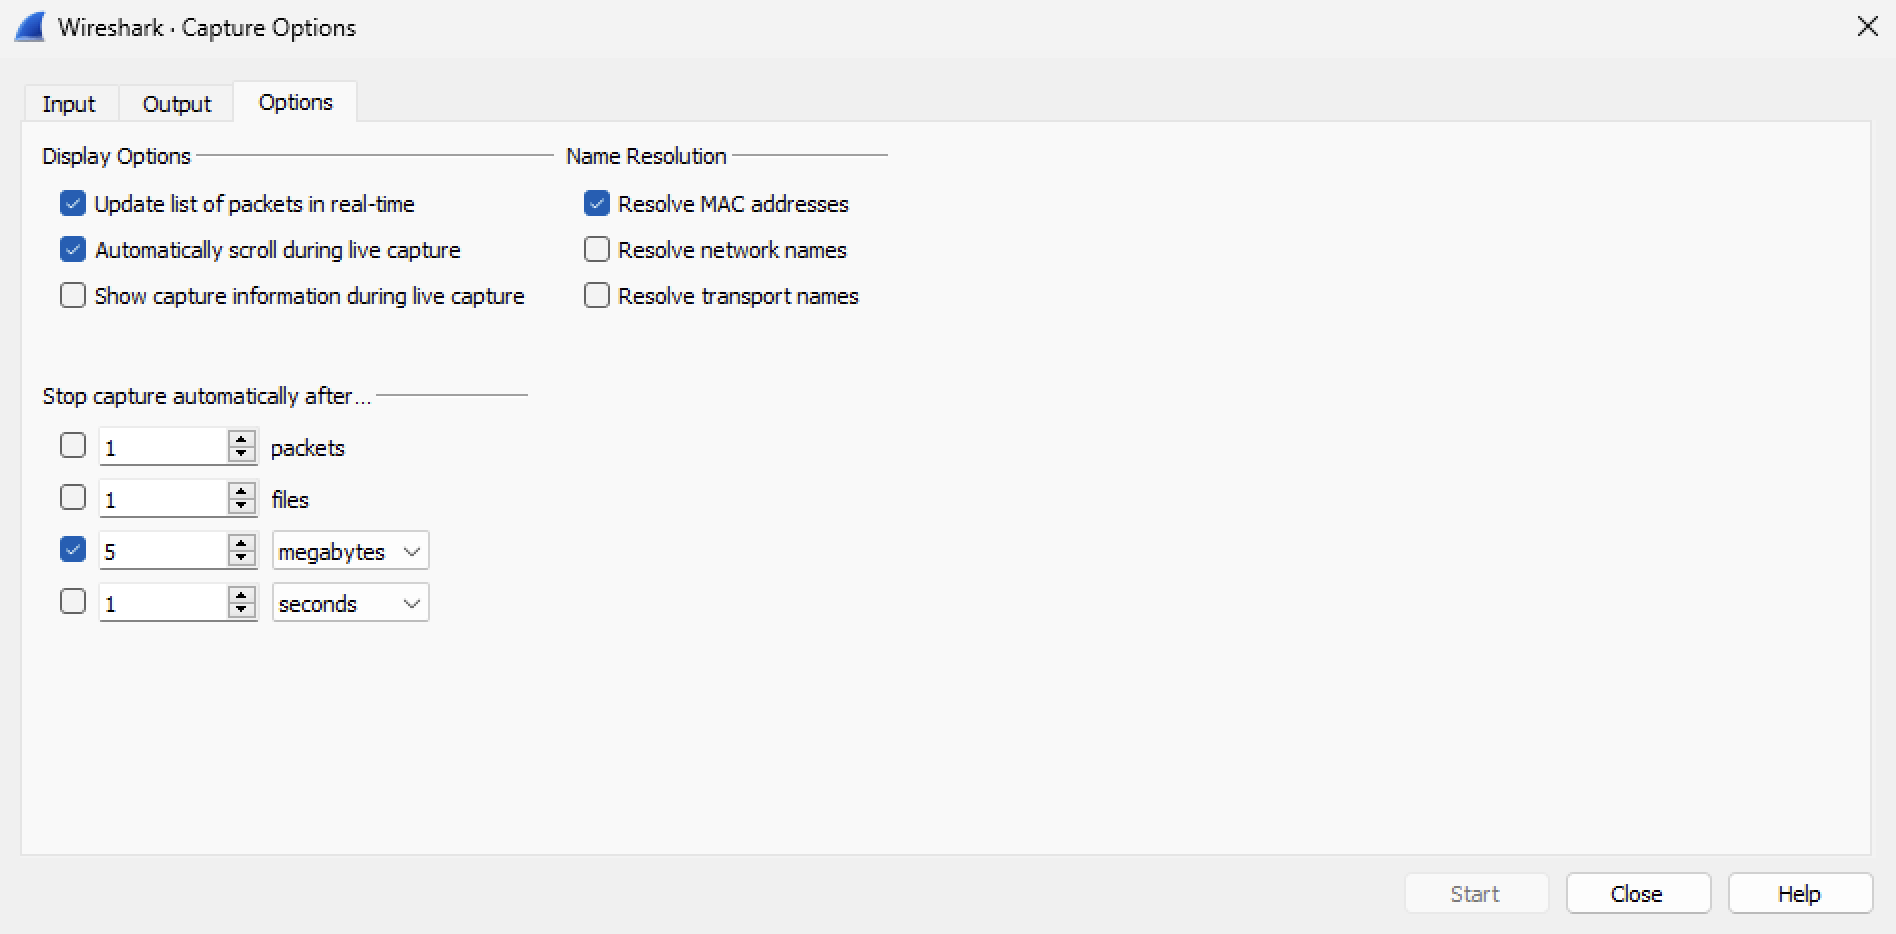
\includegraphics[width=\textwidth]{images/stop-capture-after-5-mb.png}
  \caption{Настройка автоматического завершения перехвата трафика}
  \label{fig:stop-capture-after-5-mb}
\end{figure}

Для того, чтобы настроить сохранение информации о трафике в файл, необходимо в
том же окне во вкладке <<Output>> прописать путь до директории, в котором будет
сохранен файл, а также его название (рис. \ref{fig:save-log-to-file}).

\begin{figure}[H]
  \centering
  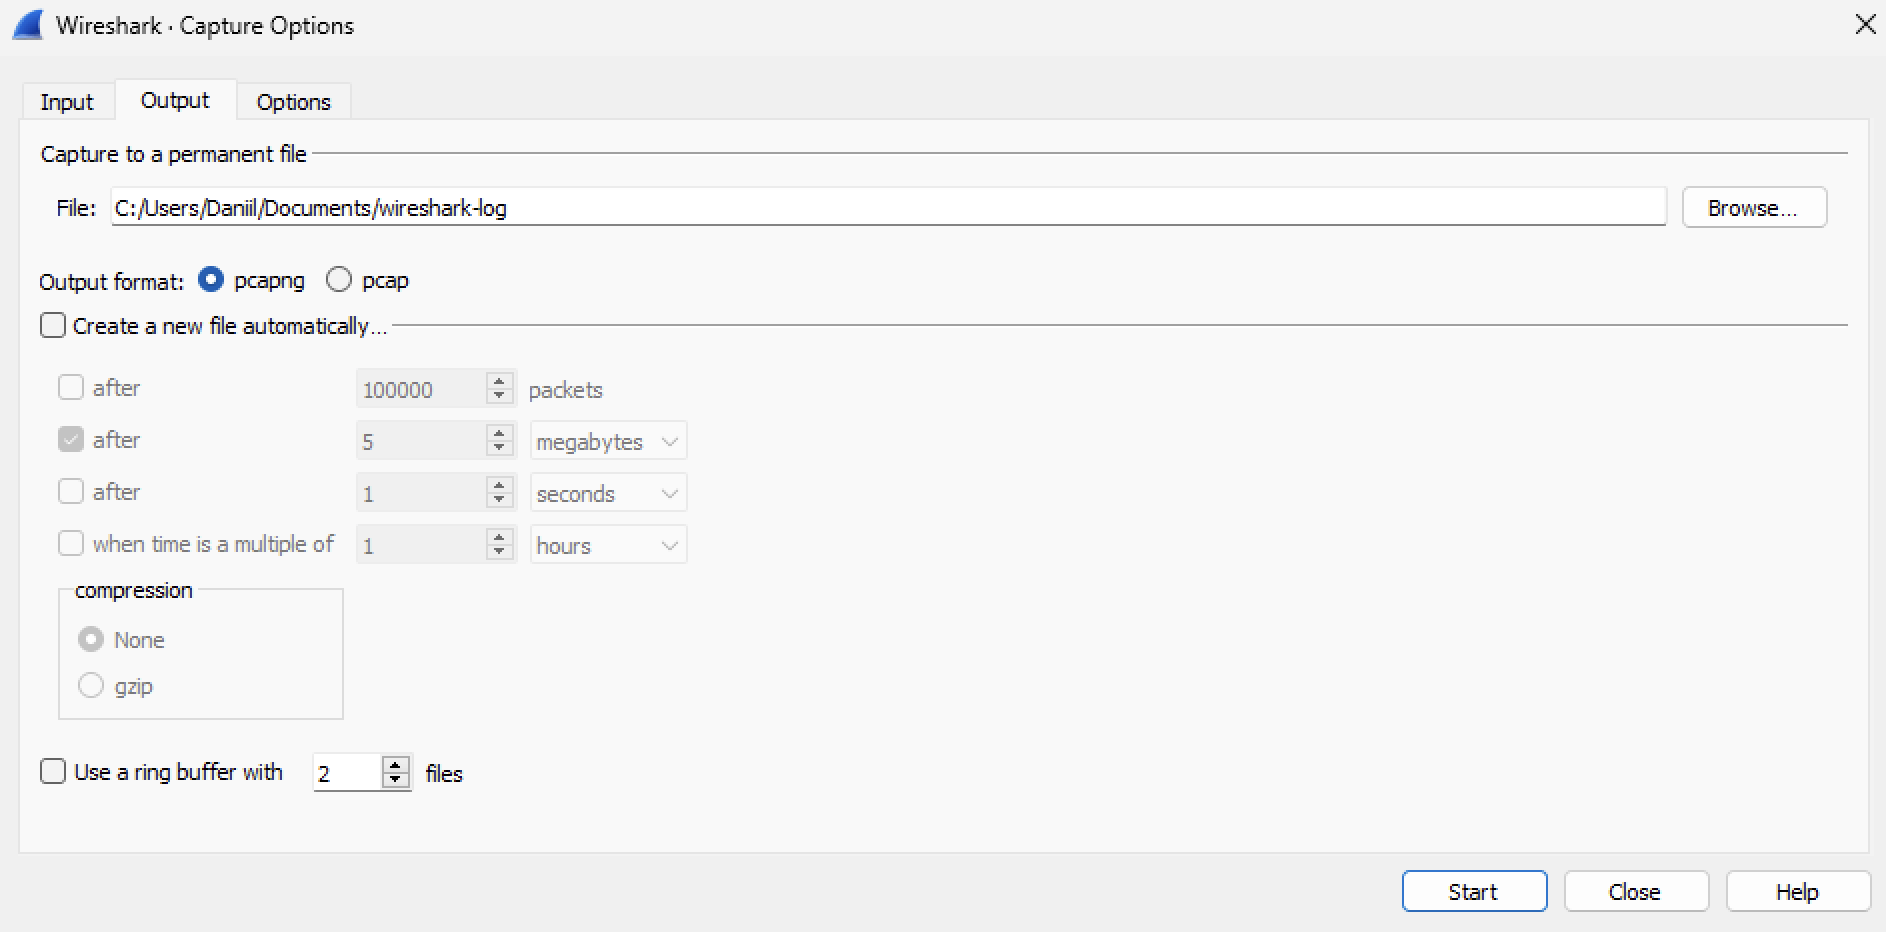
\includegraphics[width=\textwidth]{images/save-log-to-file.png}
  \caption{Настройка сохранения данных в файл}
  \label{fig:save-log-to-file}
\end{figure}

Для определения узла с максимальной активностью по объему переданных данных
необходимо на панели нажать <<Statistics>>, <<Endpoints>>. В открывшемся окне
перейти на вкладку <<IPv4>> и, поскольку активность оценивается по объему
\textbf{переданных} данных, необходимо отсортировать данный список по количеству
<<Tx Bytes>> (рис. \ref{fig:endpoints-by-tx-bytes}). В данном случае это узел с
IPv4 адресом 172.67.186.132.

\begin{figure}[H]
  \centering
  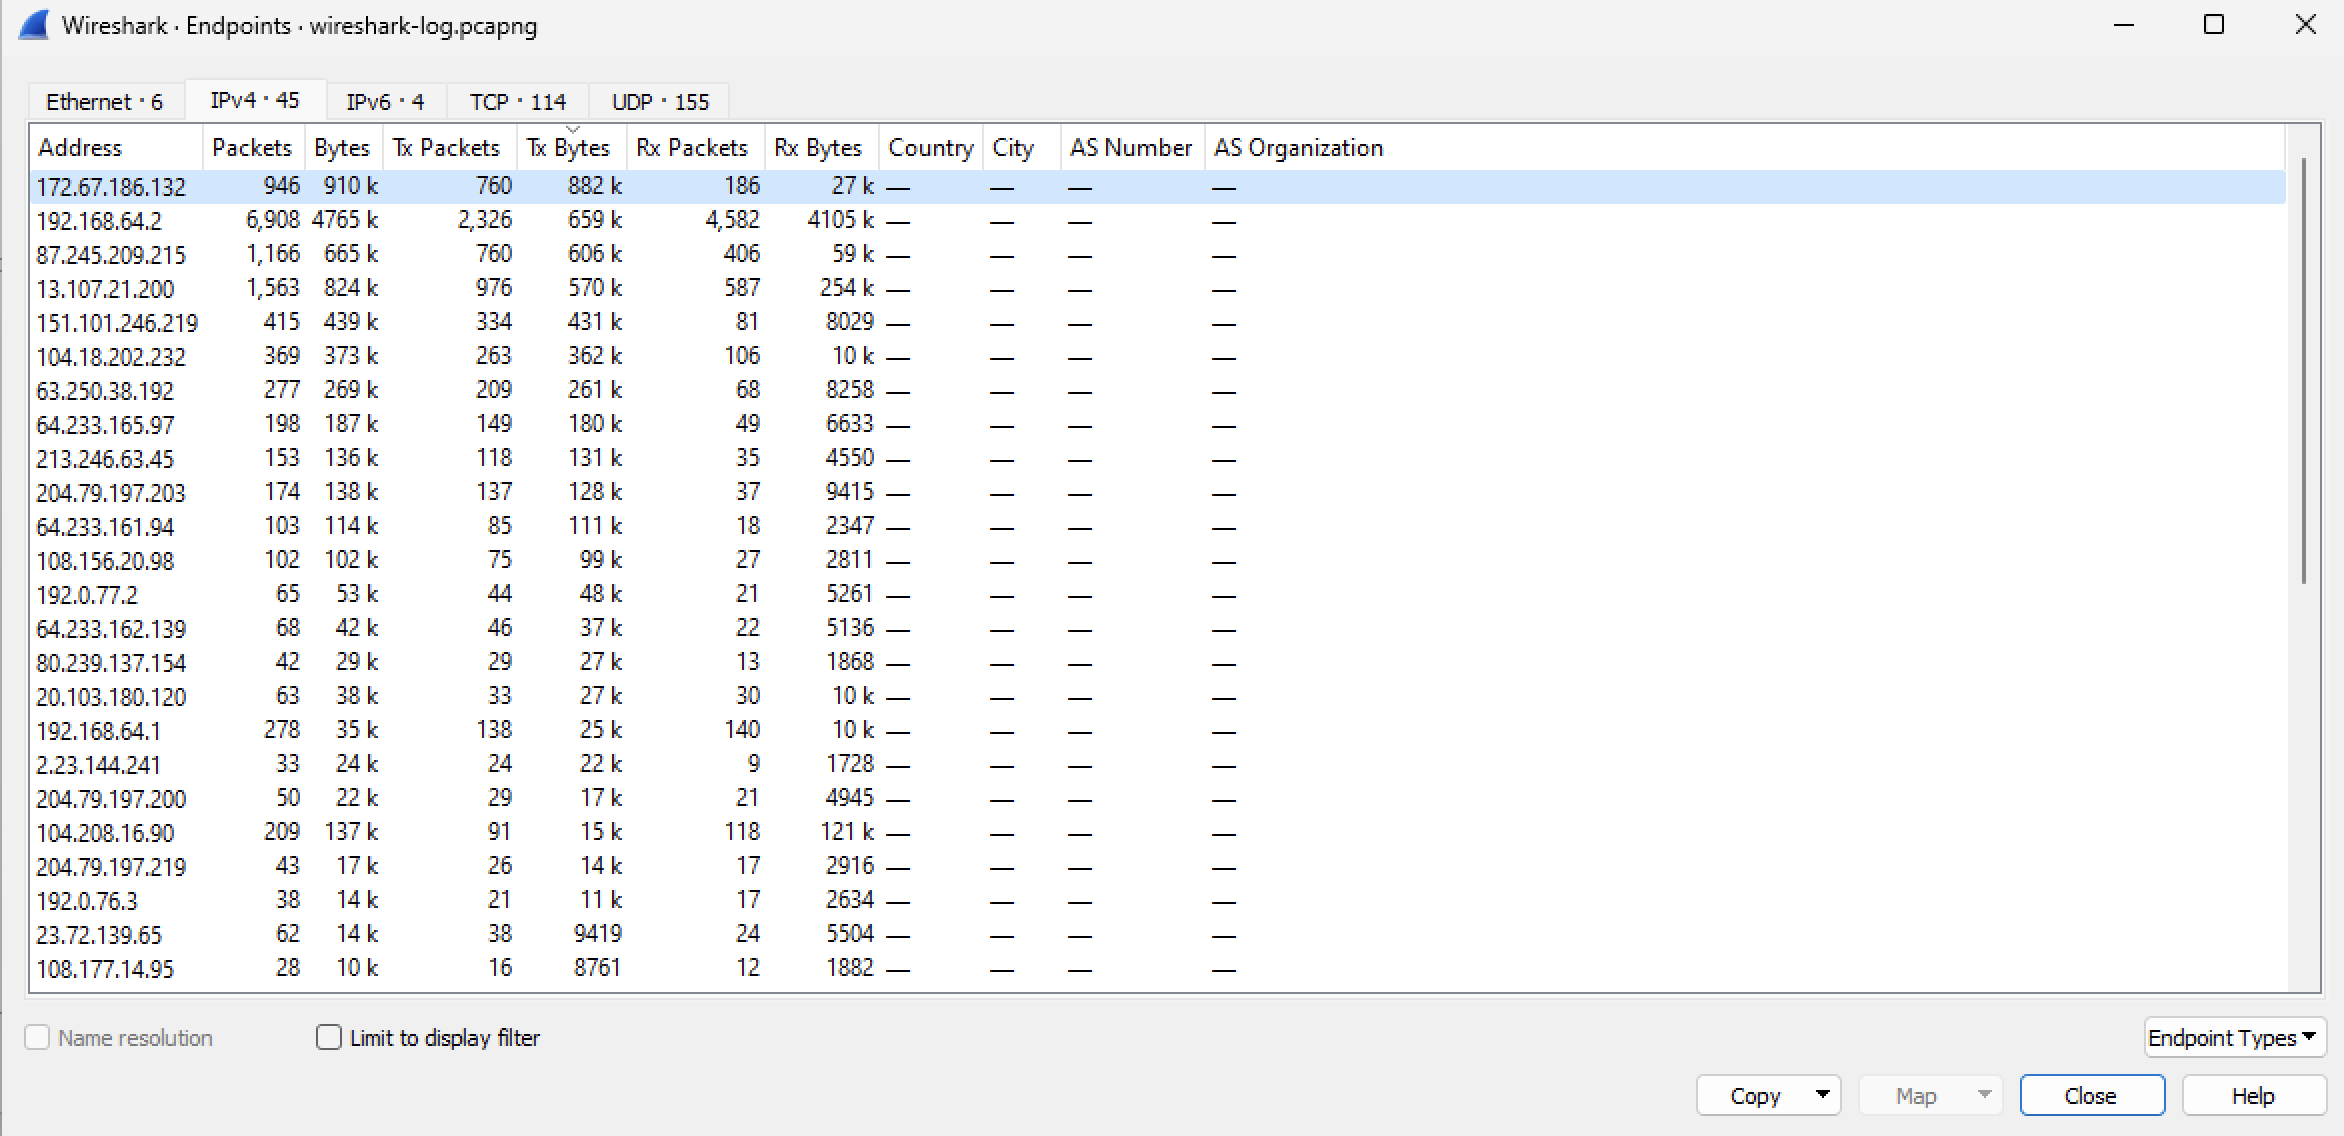
\includegraphics[width=\textwidth]{images/endpoints-by-tx-bytes.png}
  \caption{Узлы с максимальной активностью по объему переданных данных}
  \label{fig:endpoints-by-tx-bytes}
\end{figure}

Для определения самого активного TCP-порта на хосте по количеству переданных
пакетов необходимо в поле ввода ввести следующее условие фильтрации:
\begin{minted}{text}
  ip.src == 192.168.64.2
\end{minted}
Тем самым все пакеты будут отфильтрованы по адресу отправителя. В данном случае
адрес хоста равен 192.168.64.2. Затем с помощью окна <<Endpoints>>, с включенной
опцией <<Limit to display filter>>. Во вкладке <<TCP>> необходимо отсортировать
список по <<Tx Bytes>>, поскольку активность определяется по количеству
переданных пакетов. В данном случае самым активным TCP-портом является 50162
(рис. \ref{fig:tcp-by-tx-bytes}).

\begin{figure}[H]
  \centering
  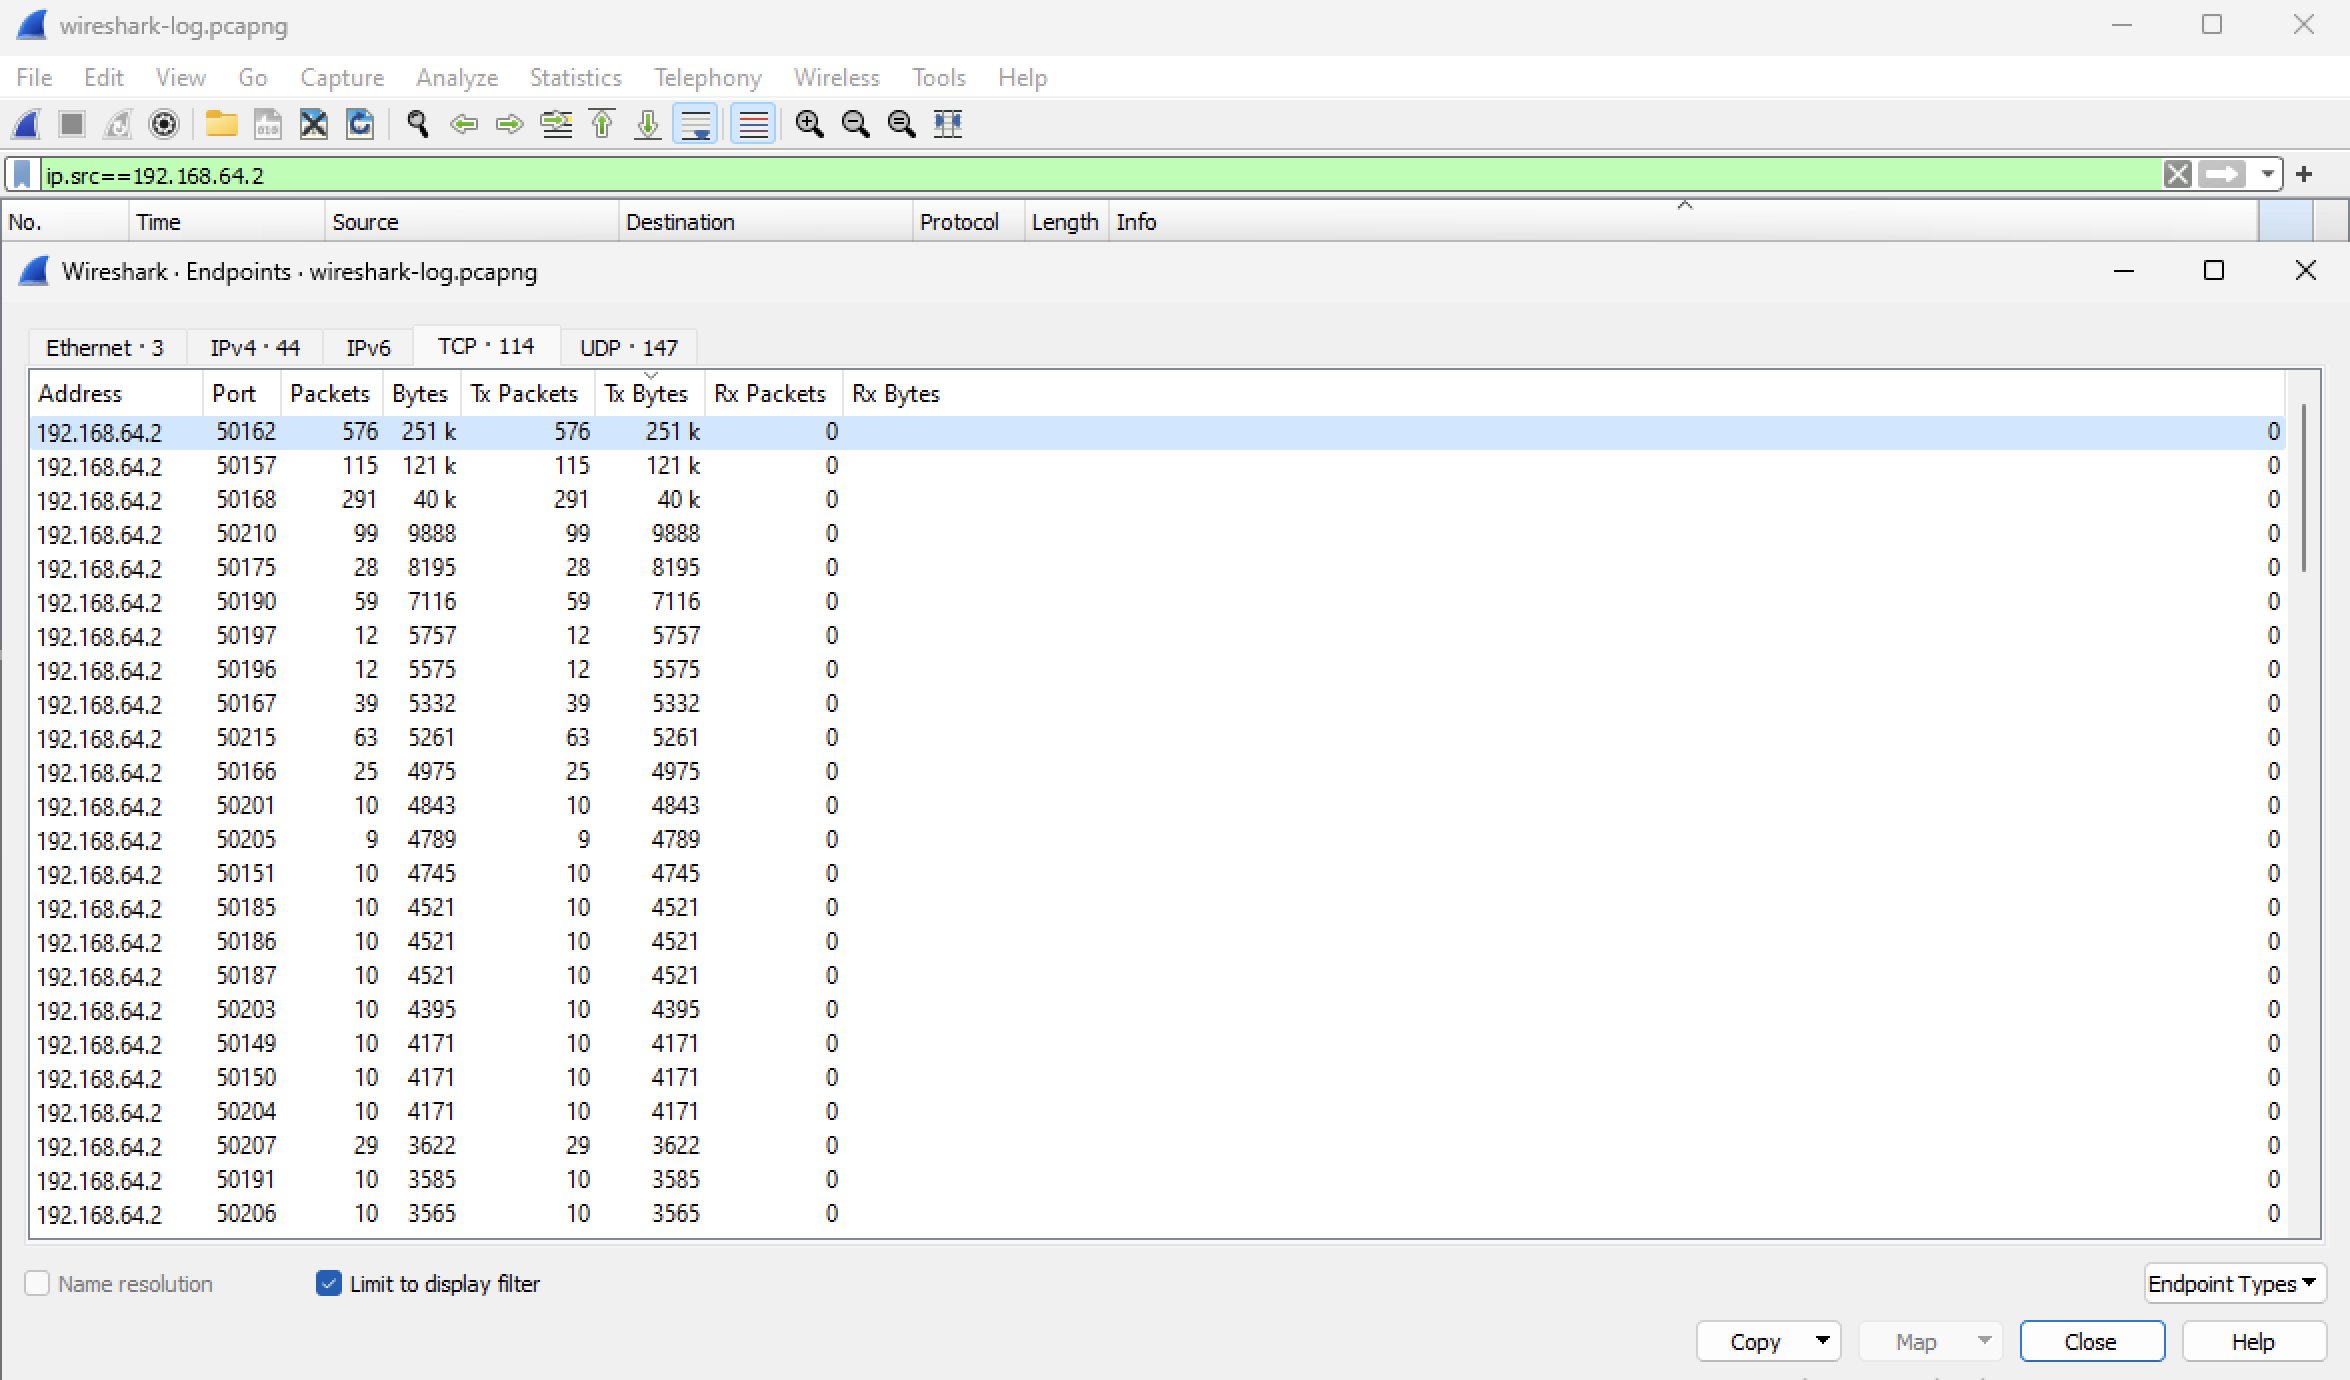
\includegraphics[width=\textwidth]{images/tcp-by-tx-bytes.png}
  \caption{Самый активный TCP-порт на хосте}
  \label{fig:tcp-by-tx-bytes}
\end{figure}

Для построения графа интенсивности TCP и UDP трафика необходимо на панели в
разделе <<Statistics>> открыть окно <<I/O Graphs>>. Там в качестве графиков
необходимо добавить два источника данных: первый с <<Display Filter>> равный
<<tcp>>, второй с <<Display Filter>> равный <<udp>> (рис.
\ref{fig:tcp-udp-graph}).

\begin{figure}[H]
  \centering
  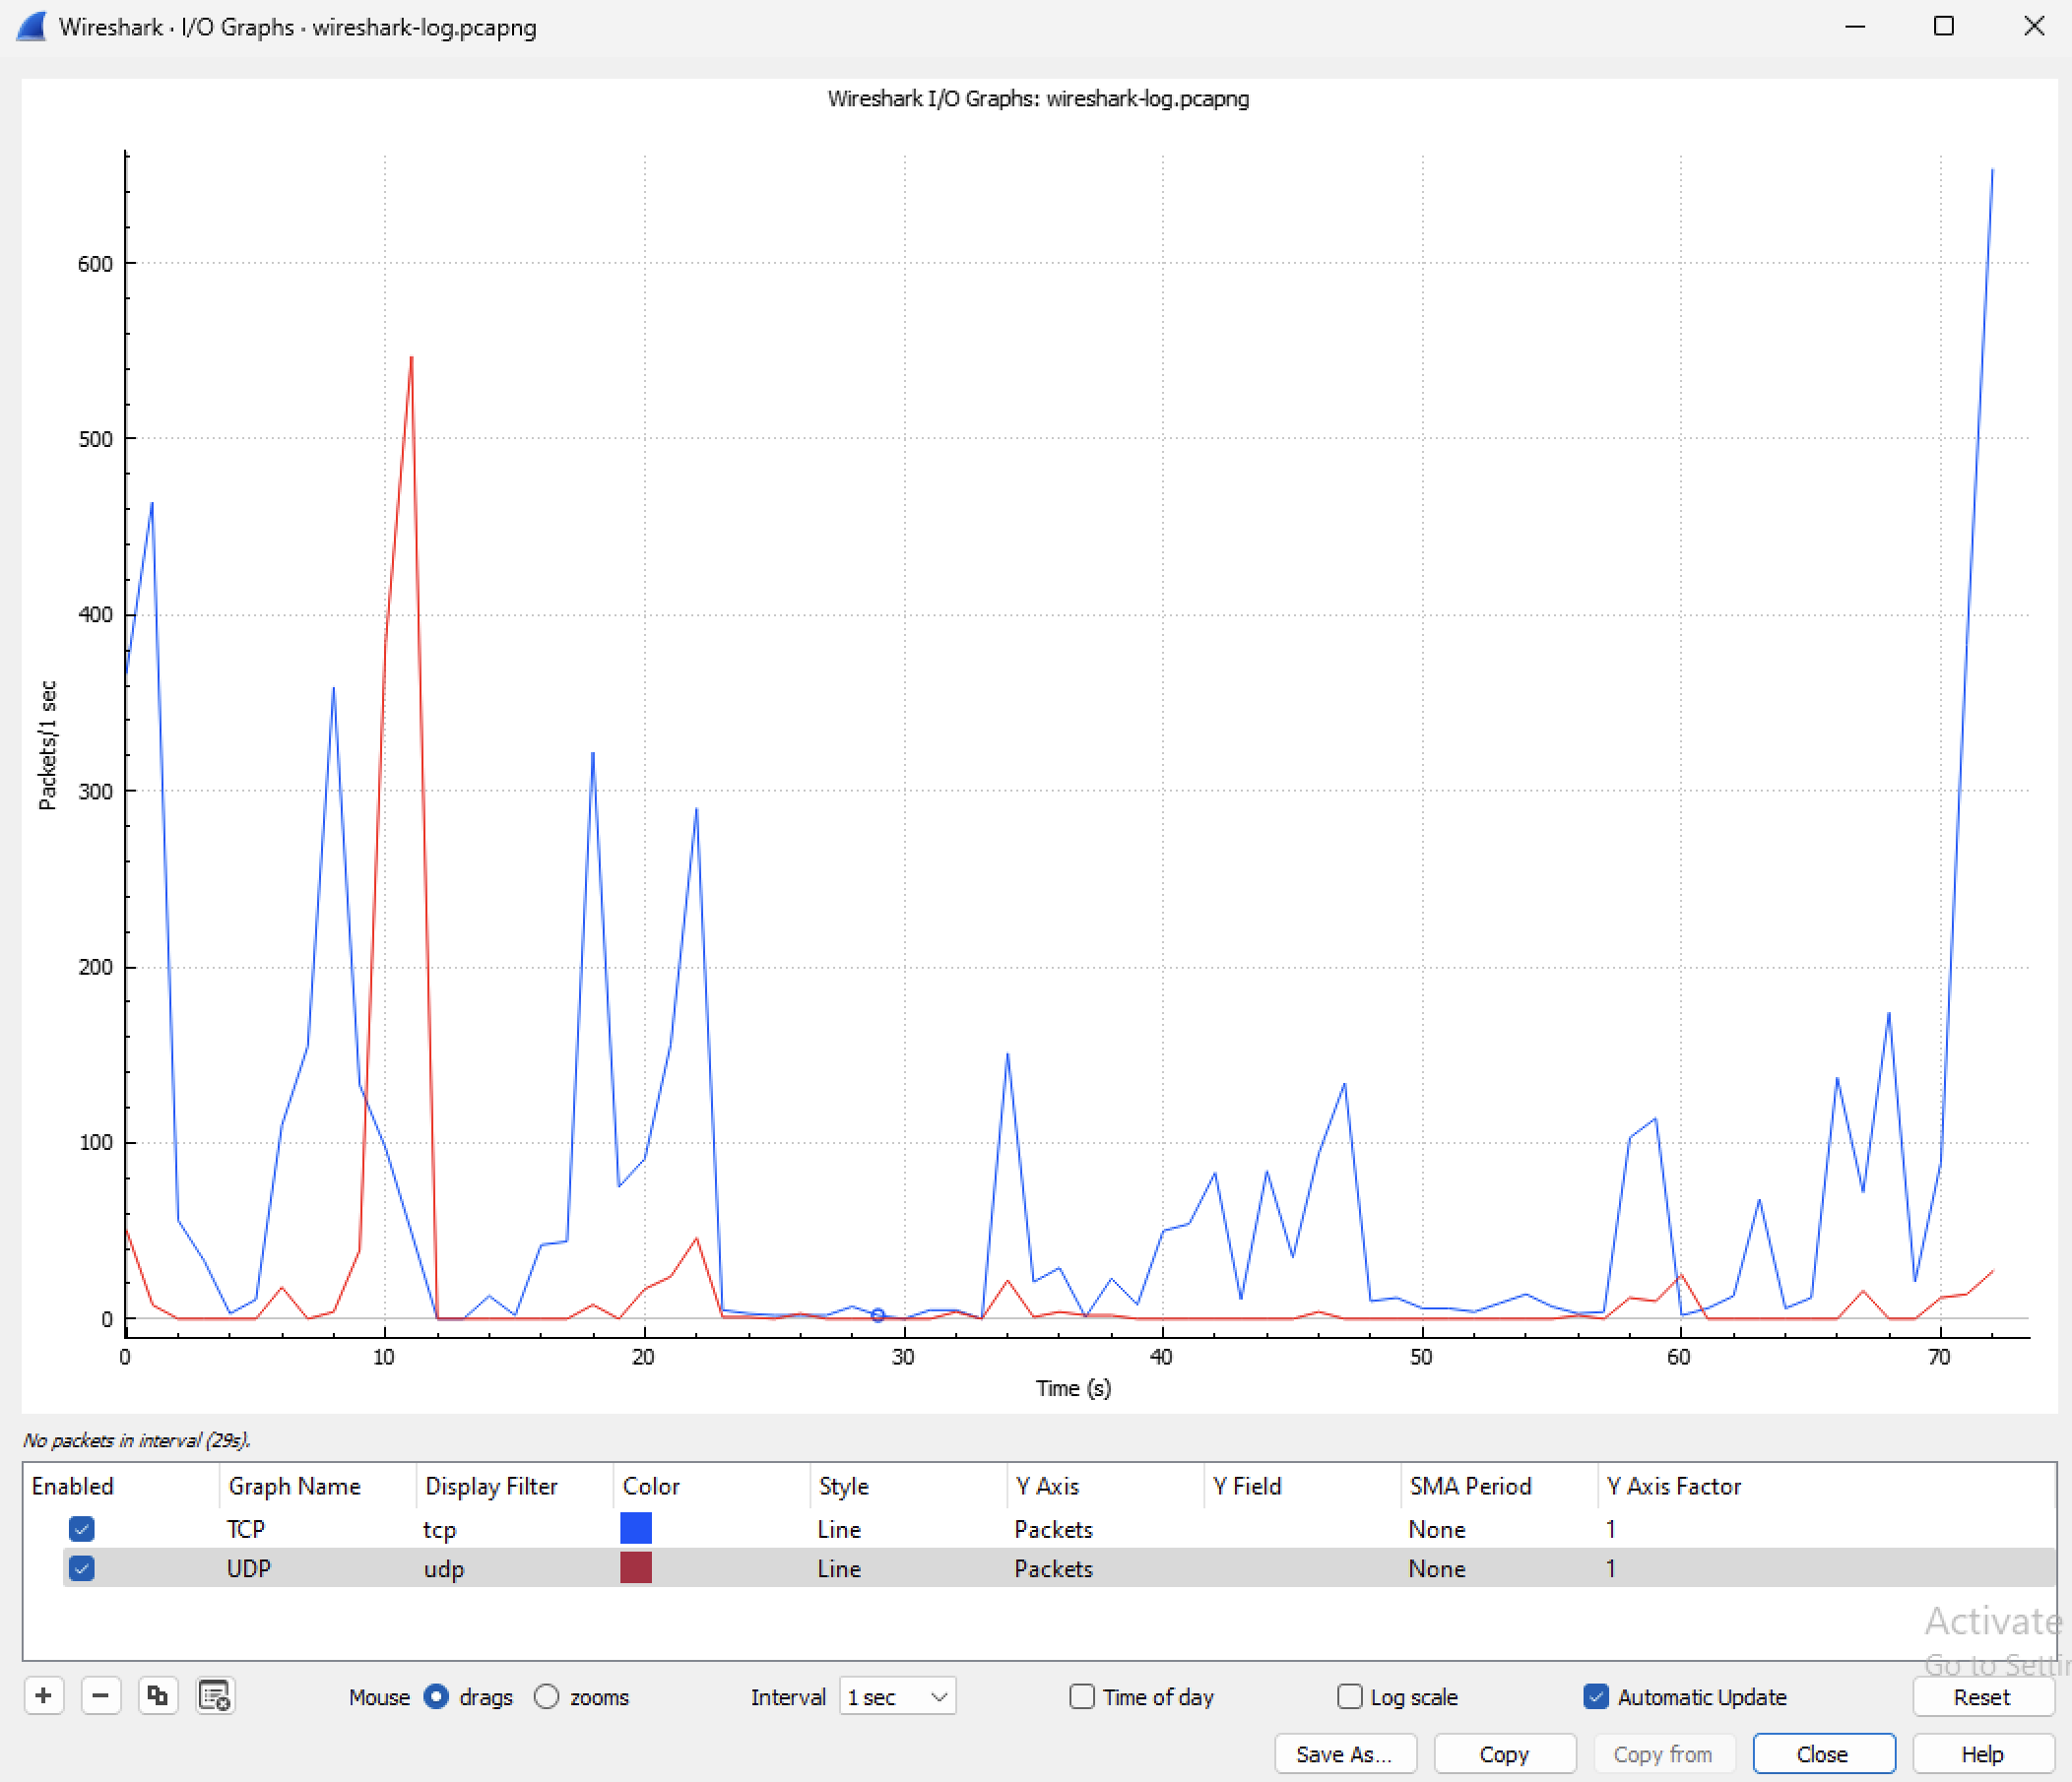
\includegraphics[width=\textwidth]{images/tcp-udp-graph.png}
  \caption{График интенсивности TCP и UDP трафика}
  \label{fig:tcp-udp-graph}
\end{figure}

Для построения диаграммы связей пакетов HTTPS необходимо в поле фильтрации
ввести следующее условие:
\begin{minted}{text}
  tcp.port==443
\end{minted}
Таким образом, поскольку HTTPS работает поверх протокола TCP на порту 443, весь
трафик будет отфильтрован по протоколу HTTPS. Затем на панели в разделе
<<Statistics>> необходимо открыть <<Flow graph>>. В открывшемся окне необходимо
включить опцию <<Limit to display filter>>, а также в выпадающем поле <<Flow
type>> выбрать <<TCP Flows>>. Тем самым будет построена диаграмма связей для
HTTPS пакетов (рис. \ref{fig:https-flow-graph}).

\begin{figure}[H]
  \centering
  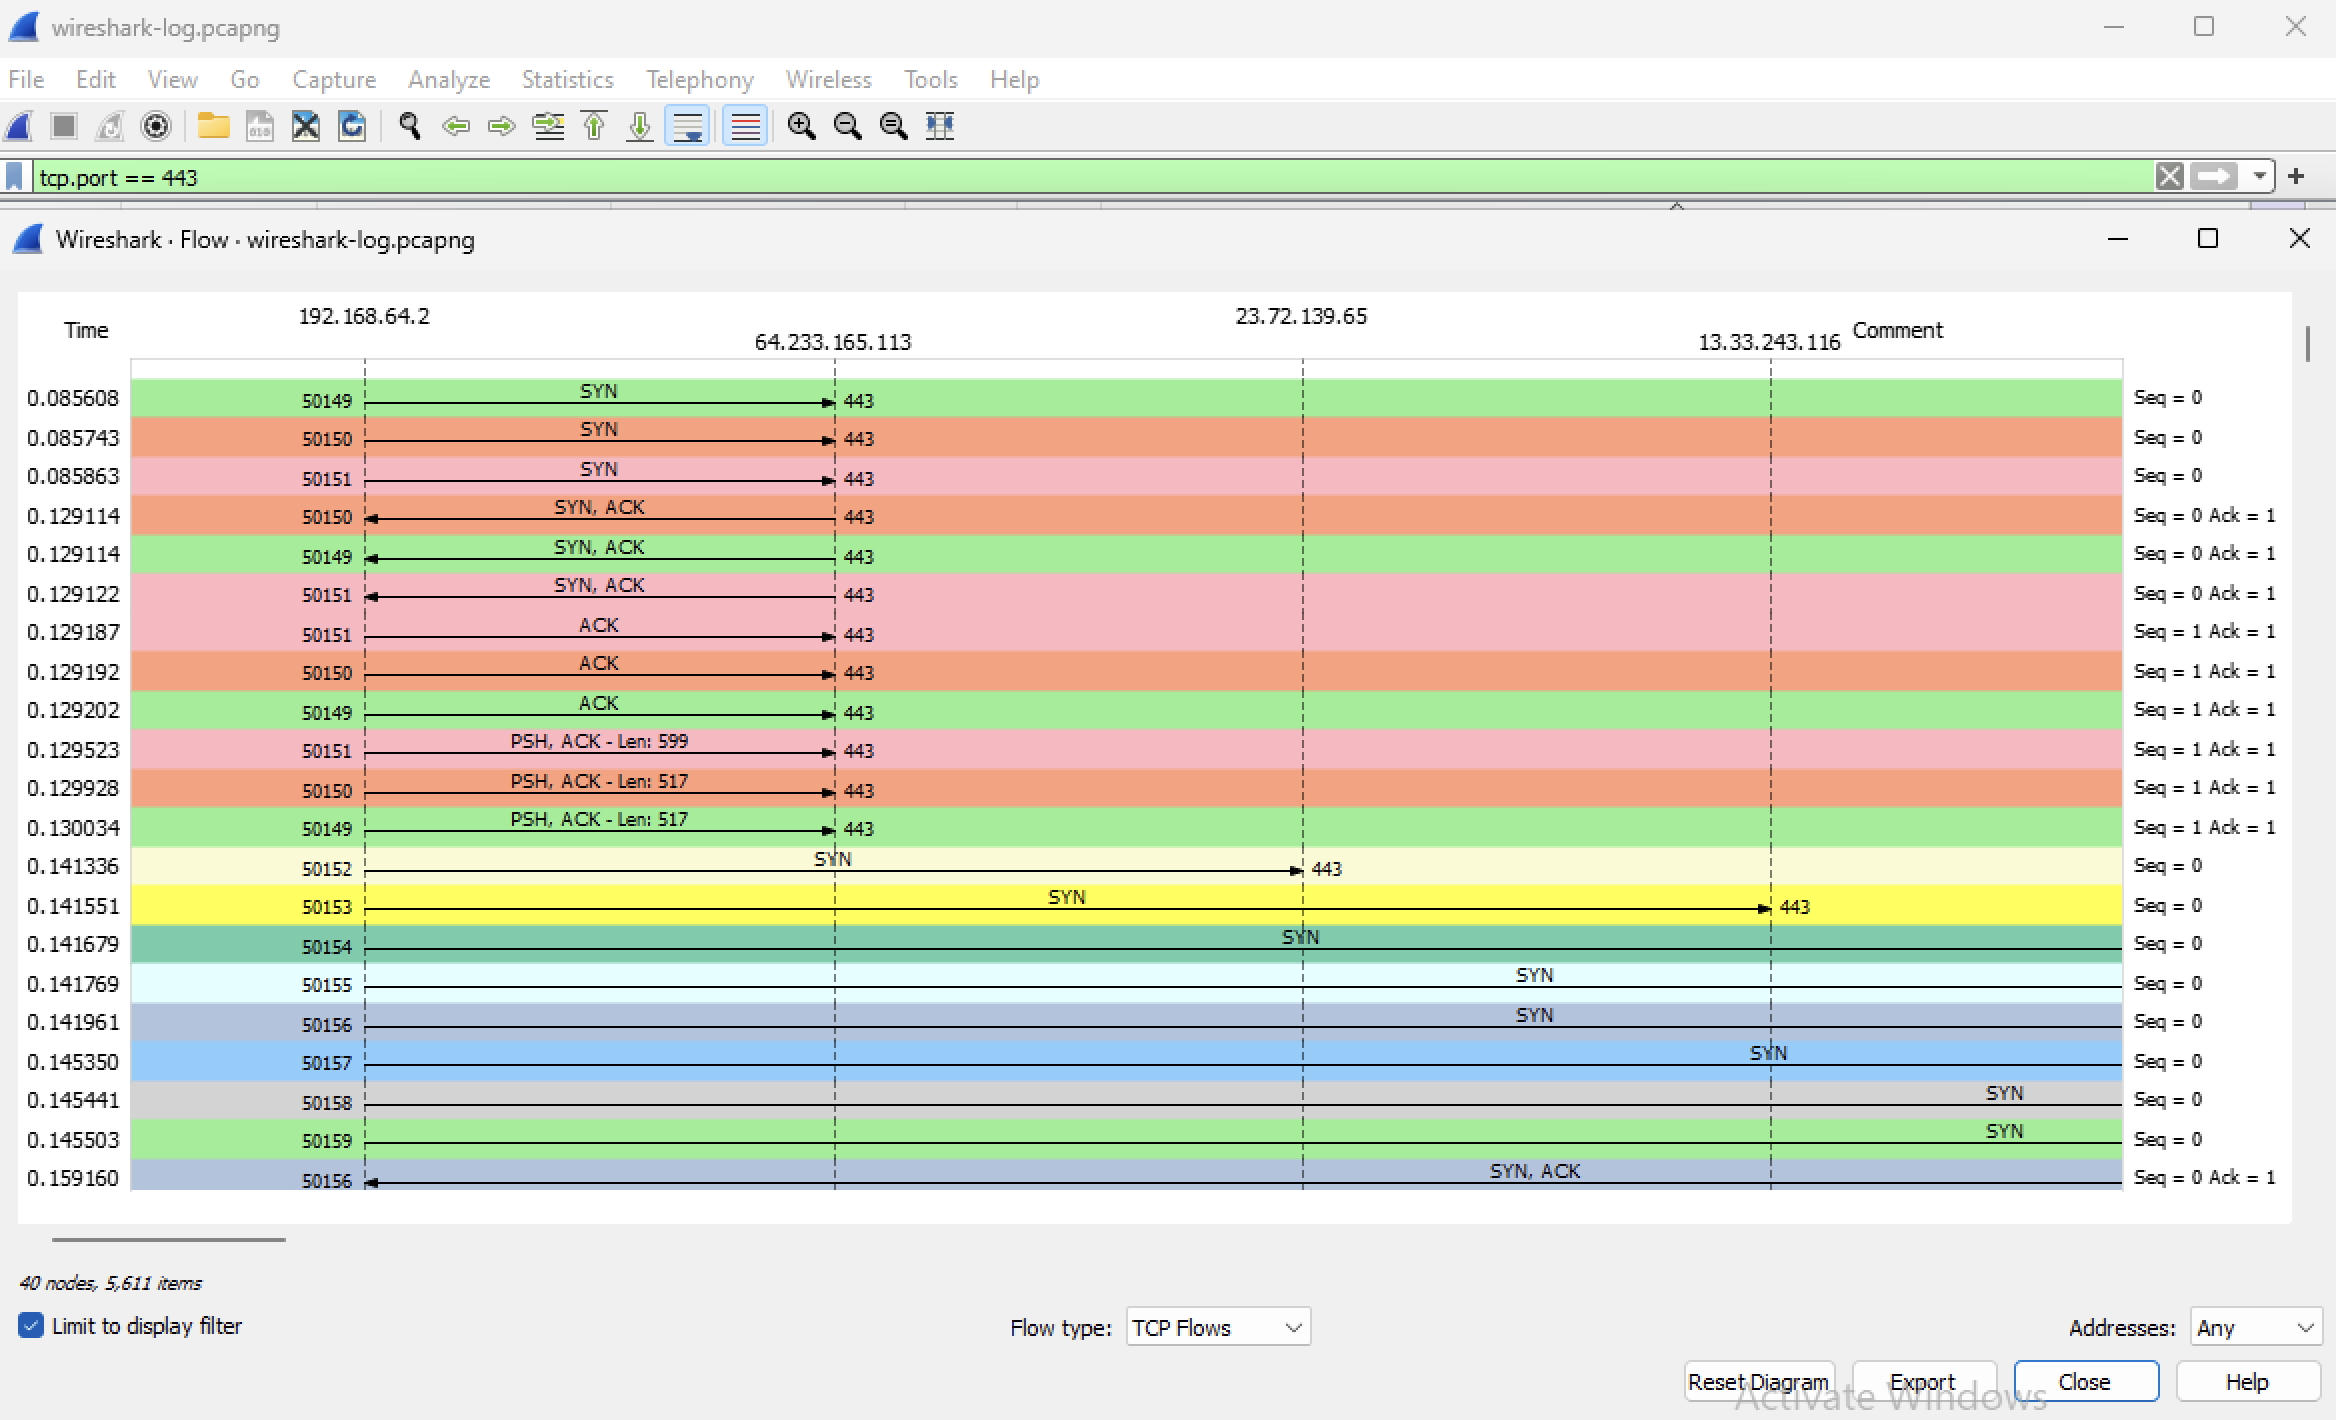
\includegraphics[width=\textwidth]{images/https-flow-graph.png}
  \caption{Диаграмма связей HTTPS пакетов}
  \label{fig:https-flow-graph}
\end{figure}

В моем случае не было зафиксировано HTTP трафика, поэтому для фильтрации
использовался протокол HTTPS. Для фильтрации HTTP трафика достаточно изменить
TCP-порт с 443 на 80. Для того, чтобы отфильтровать HTTPS трафик только для
клиента, исключив пакеты к серверу, воспользуемся следующим фильтром:
\begin{minted}{text}
  (tcp.dstport == 443 and ip.src == 192.168.64.2) or
  (tcp.srcport == 443 and ip.dst == 192.168.64.2)
\end{minted}
В данном фильтре выбирается весь трафик, который либо отправляется хостом на
внешний сервер на порт 443, либо отправляется внешним сервером с порта 443 на
адрес хоста. В данный фильтр не попадет трафик сервера, поскольку сервер либо
отправляет с 443 порта на порт, отличный от 443, либо принимает на 443 порт с
порта, отличного от 443.

Для фильтрации всех кадров Ethernet, отправленных с сетевого интерфейса хоста,
необходимо воспользоваться следующим фильтром:
\begin{minted}{text}
  eth.src == 7a:12:3e:a9:df:a1
\end{minted}
Тем самым, поскольку в данном случае MAC-адрес хоста равен 7a:12:3e:a9:df:a1,
будут показаны только пакеты, отправляемые с сетевого интерфейса хоста (рис.
\ref{fig:eth-src}).

\begin{figure}[H]
  \centering
  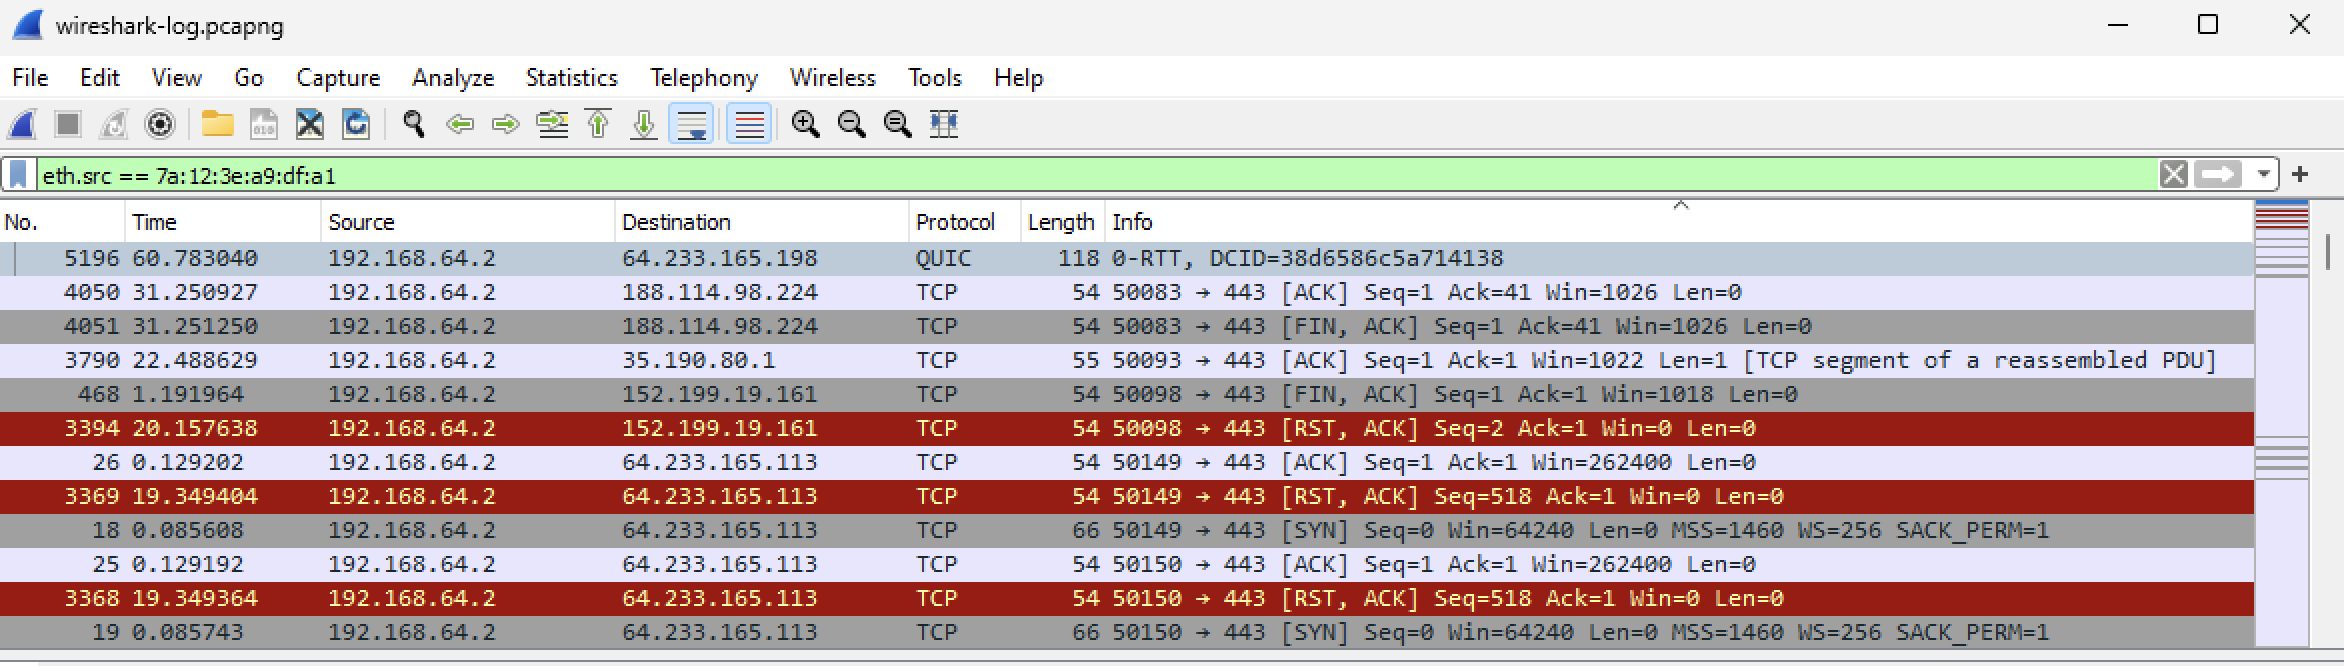
\includegraphics[width=\textwidth]{images/eth-src.png}
  \caption{Кадры Ethernet, отправляемые с сетевого интерфейса хоста}
  \label{fig:eth-src}
\end{figure}

Для того, чтобы отфильтровать только широковещательные сообщения, необходимо
использовать следующий фильтр:
\begin{minted}{text}
  eth.dst == ff:ff:ff:ff:ff:ff
\end{minted}
Таким образом будут показаны только те пакеты, которые были отправлены на
широковещательный адрес. Как видно на рис. \ref{fig:broadcast}, среди
протоколов, есть только UDP.

\begin{figure}[H]
  \centering
  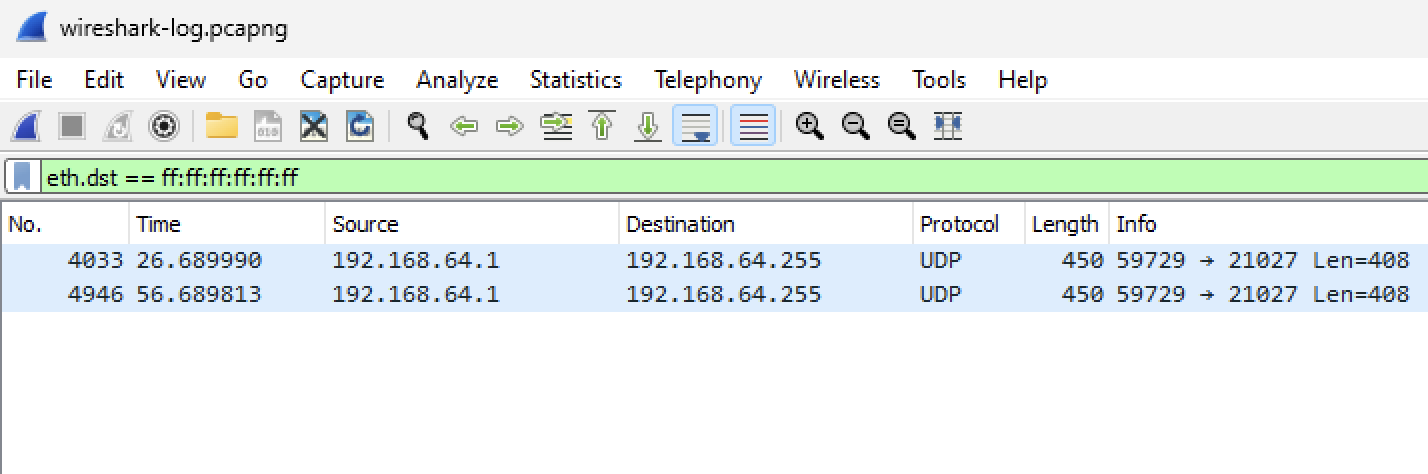
\includegraphics[width=\textwidth]{images/broadcast.png}
  \caption{Список широковещательных сообщений}
  \label{fig:broadcast}
\end{figure}

Исходя из того, что широковещательных рассылок было достаточно мало, можно
сказать, что устройство было подключено к маршрутизатору.

\subsection{Сбор и анализ данных протокола ICMP}

Для разрешения ICMP-запросов в Windows необходимо настроить брандмауэр. Для
этого нужно создать новое Inbound правило (рис. \ref{fig:firewall-icmp-1}),
которое будет пропускать все входящие пакеты по протоколу ICMPv4 (рис.
\ref{fig:firewall-icmp-2} и \ref{fig:firewall-icmp-3}).

\begin{figure}[H]
  \centering
  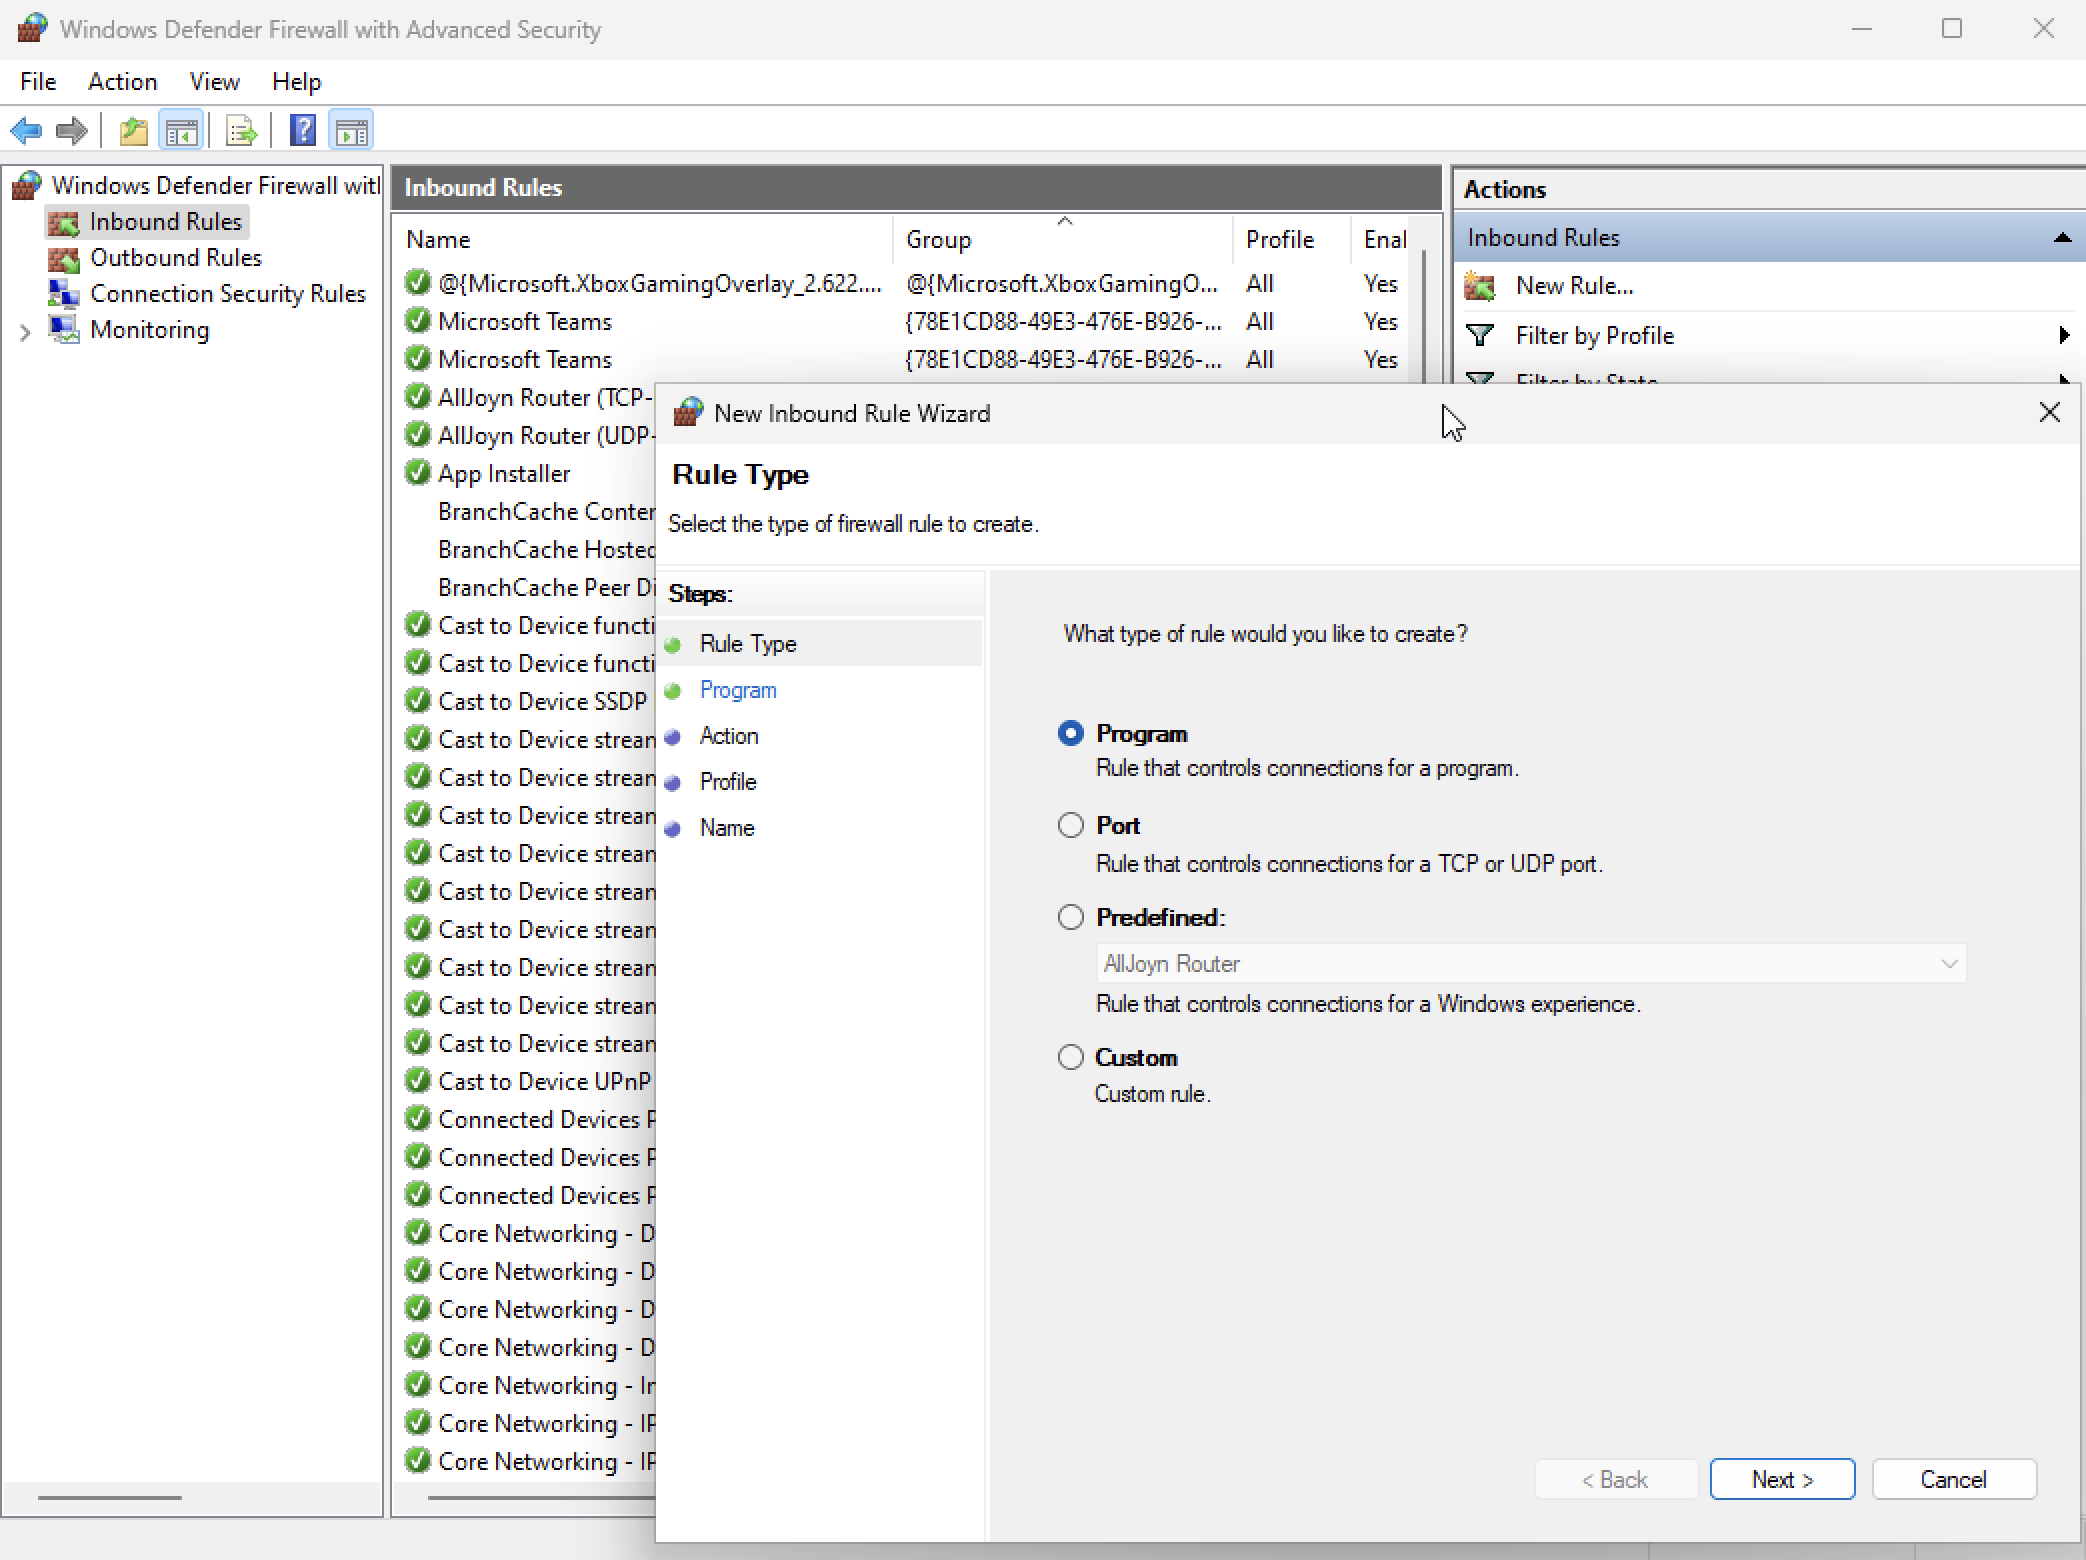
\includegraphics[width=\textwidth]{images/firewall-icmp-1.png}
  \caption{Создание нового правила в брандмауэре Windows}
  \label{fig:firewall-icmp-1}
\end{figure}

\begin{figure}[H]
  \centering
  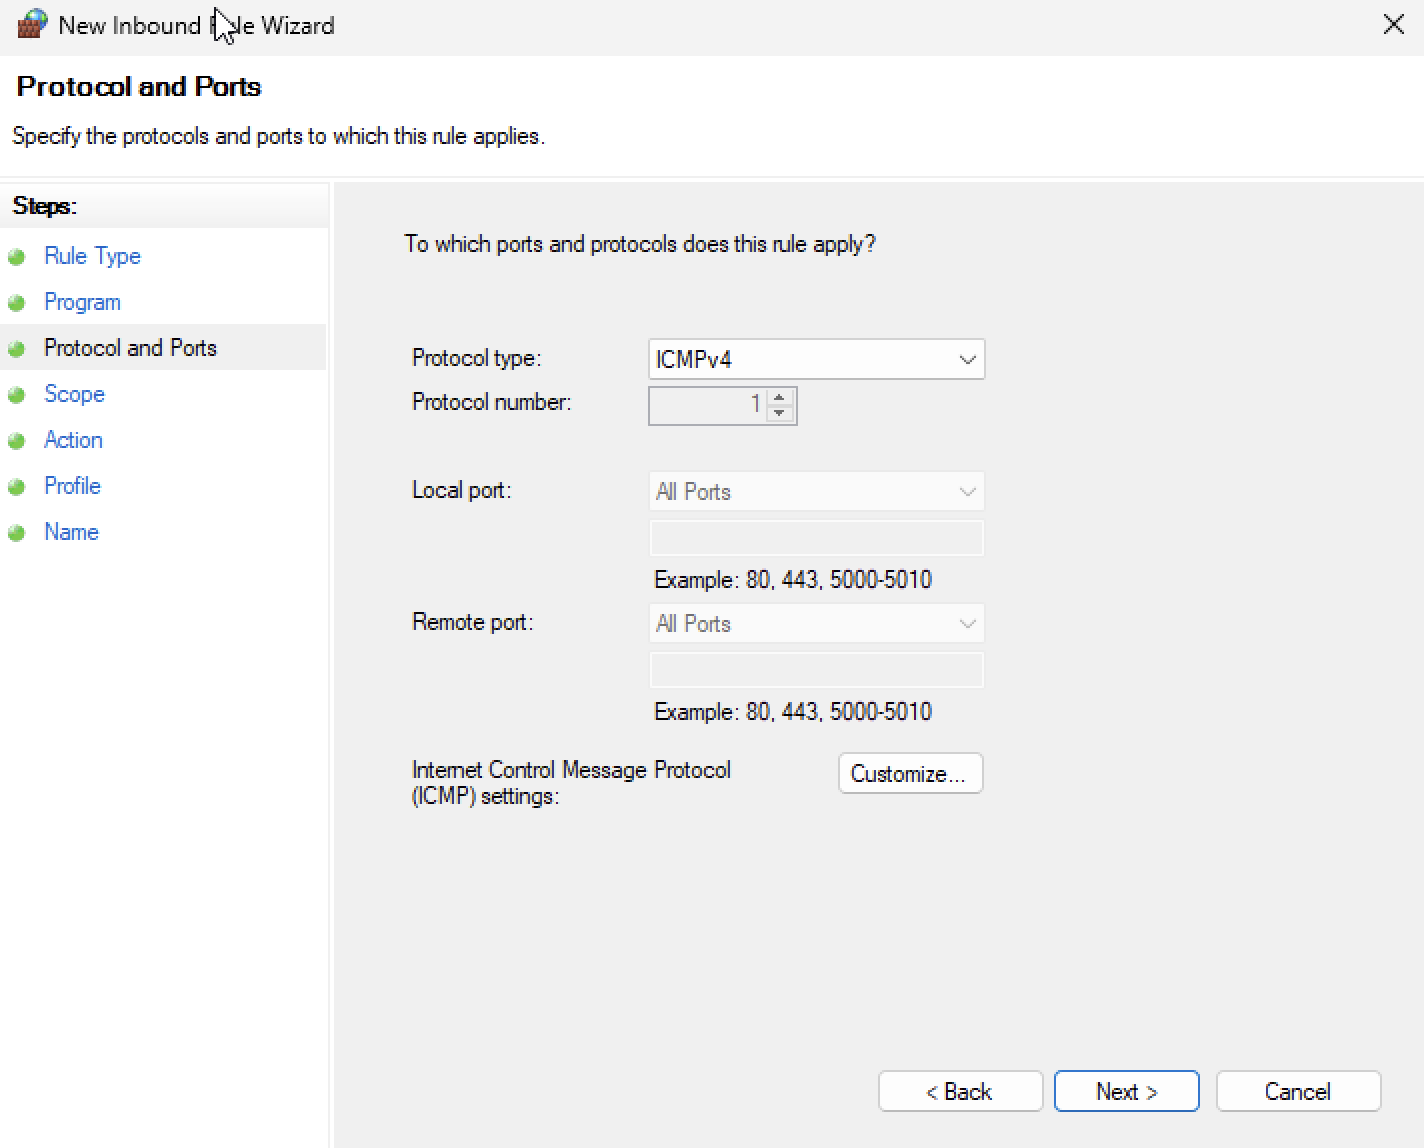
\includegraphics[width=0.75\textwidth]{images/firewall-icmp-2.png}
  \caption{Выбор протокола при создании нового правила}
  \label{fig:firewall-icmp-2}
\end{figure}

\begin{figure}[H]
  \centering
  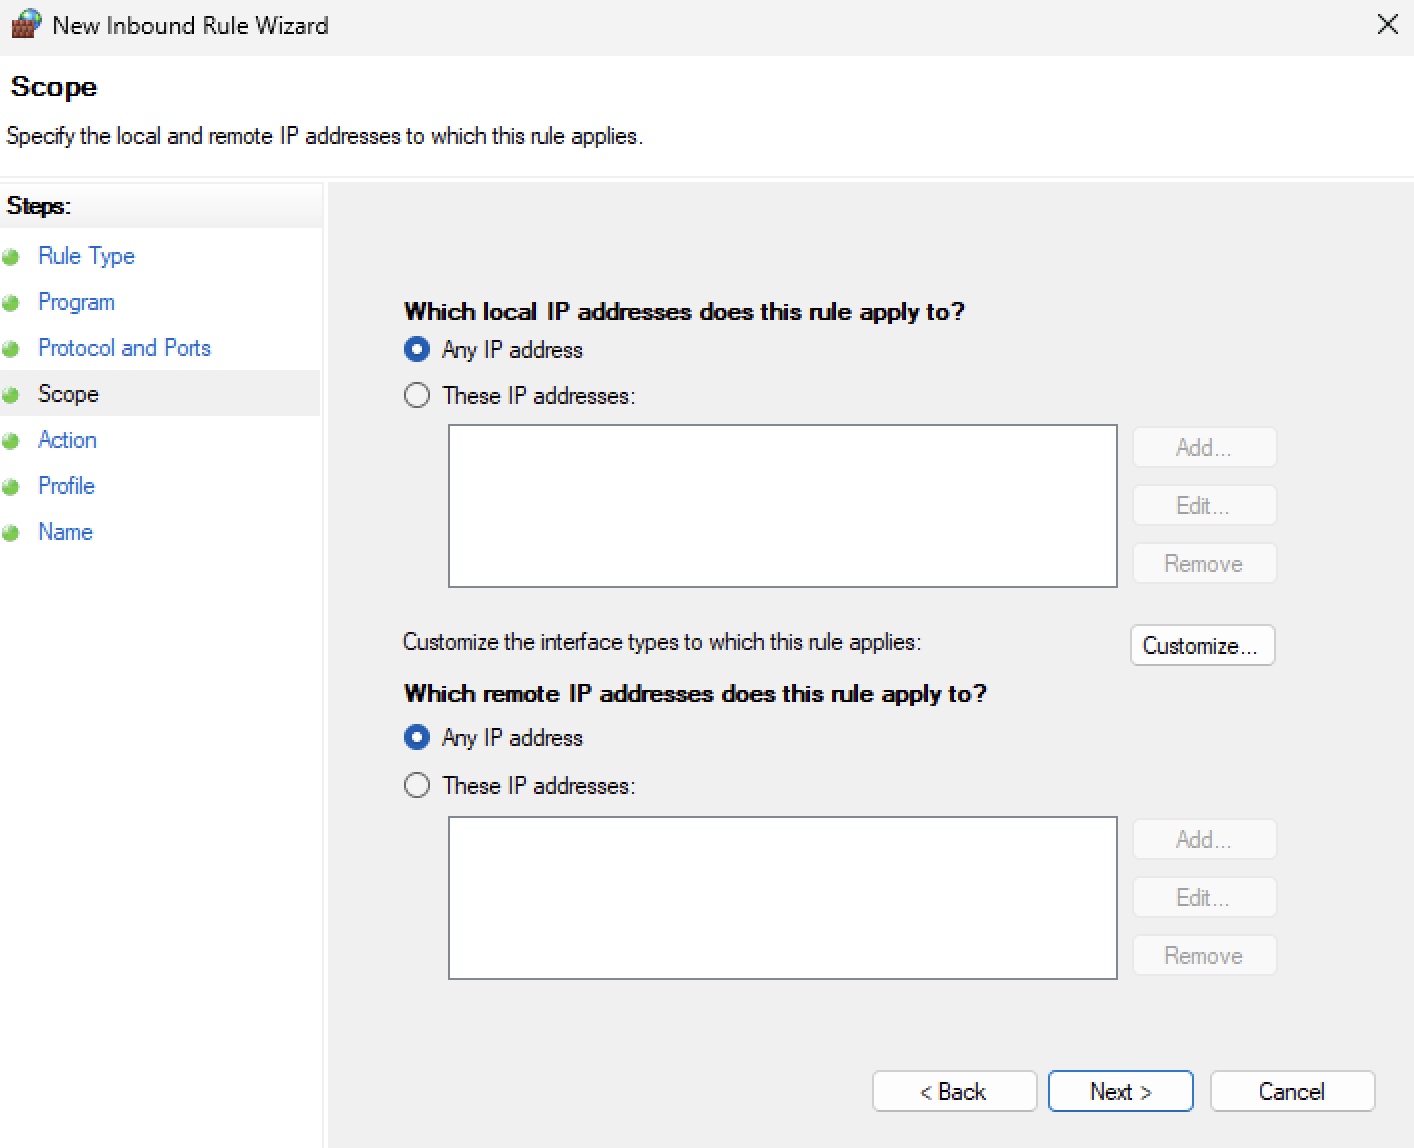
\includegraphics[width=0.75\textwidth]{images/firewall-icmp-3.png}
  \caption{Разрешение входящих запросов с любого IP-адреса}
  \label{fig:firewall-icmp-3}
\end{figure}

В качестве локального устройства, которому будут отправляться ICMP запросы, был
выбран компьютер с IP-адресом 192.168.1.254. Хост, в свою очередь, имеет адрес
IP-адрес 192.168.1.101.

Для фильтрации ICMP-пакетов, отправляемых при ping-запросе, необходимо
использовать следующий фильтр:
\begin{minted}{text}
  icmp
\end{minted}

После запуска перехвата пакетов в Wireshark, а также после запуска утилиты ping
на другом локальном компьютере (рис. \ref{fig:ping}), через некоторое время в
окне Wireshark появится информация о перехваченных ICMP-пакетах (рис.
\ref{fig:icmp-result}). Как можно видеть, IP-адреса отправителя и получателя
соответствуют адресам компьютеров отправителя и получателя.

\begin{figure}[H]
  \centering
  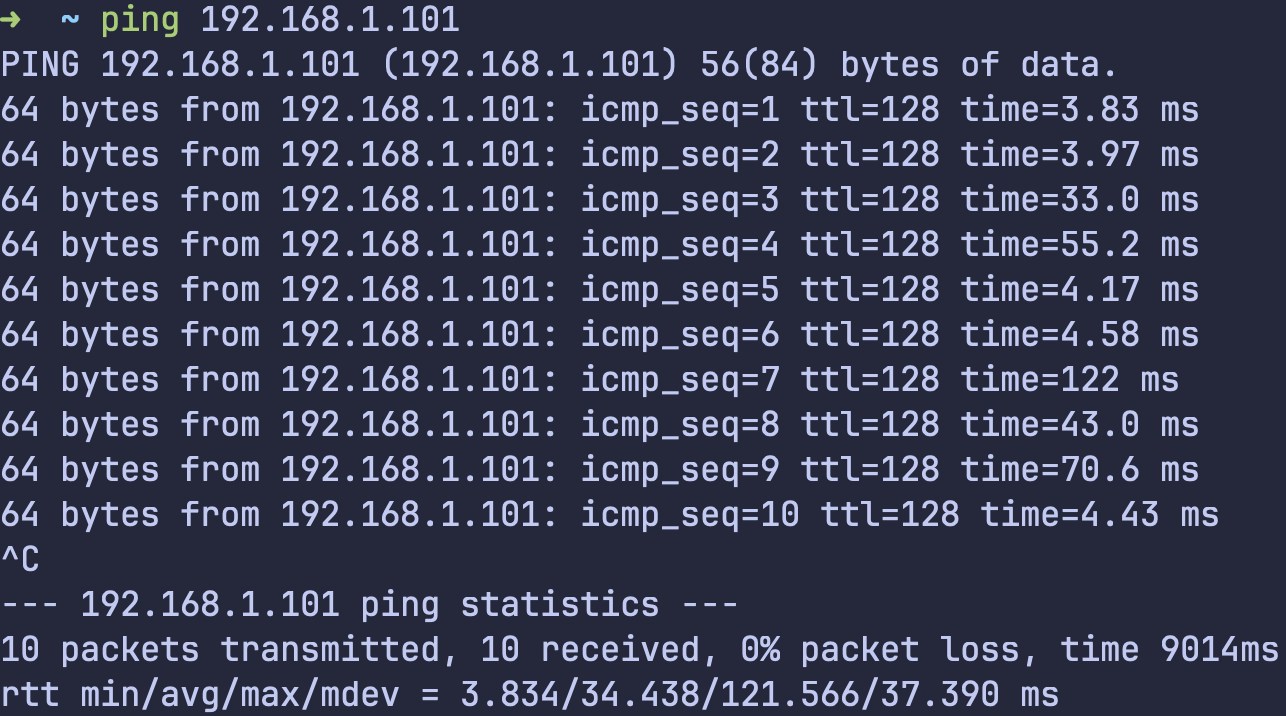
\includegraphics[width=0.5\textwidth]{images/ping.png}
  \caption{Создание ICMP-запроса с помощью утилиты ping}
  \label{fig:ping}
\end{figure}

\begin{figure}[H]
  \centering
  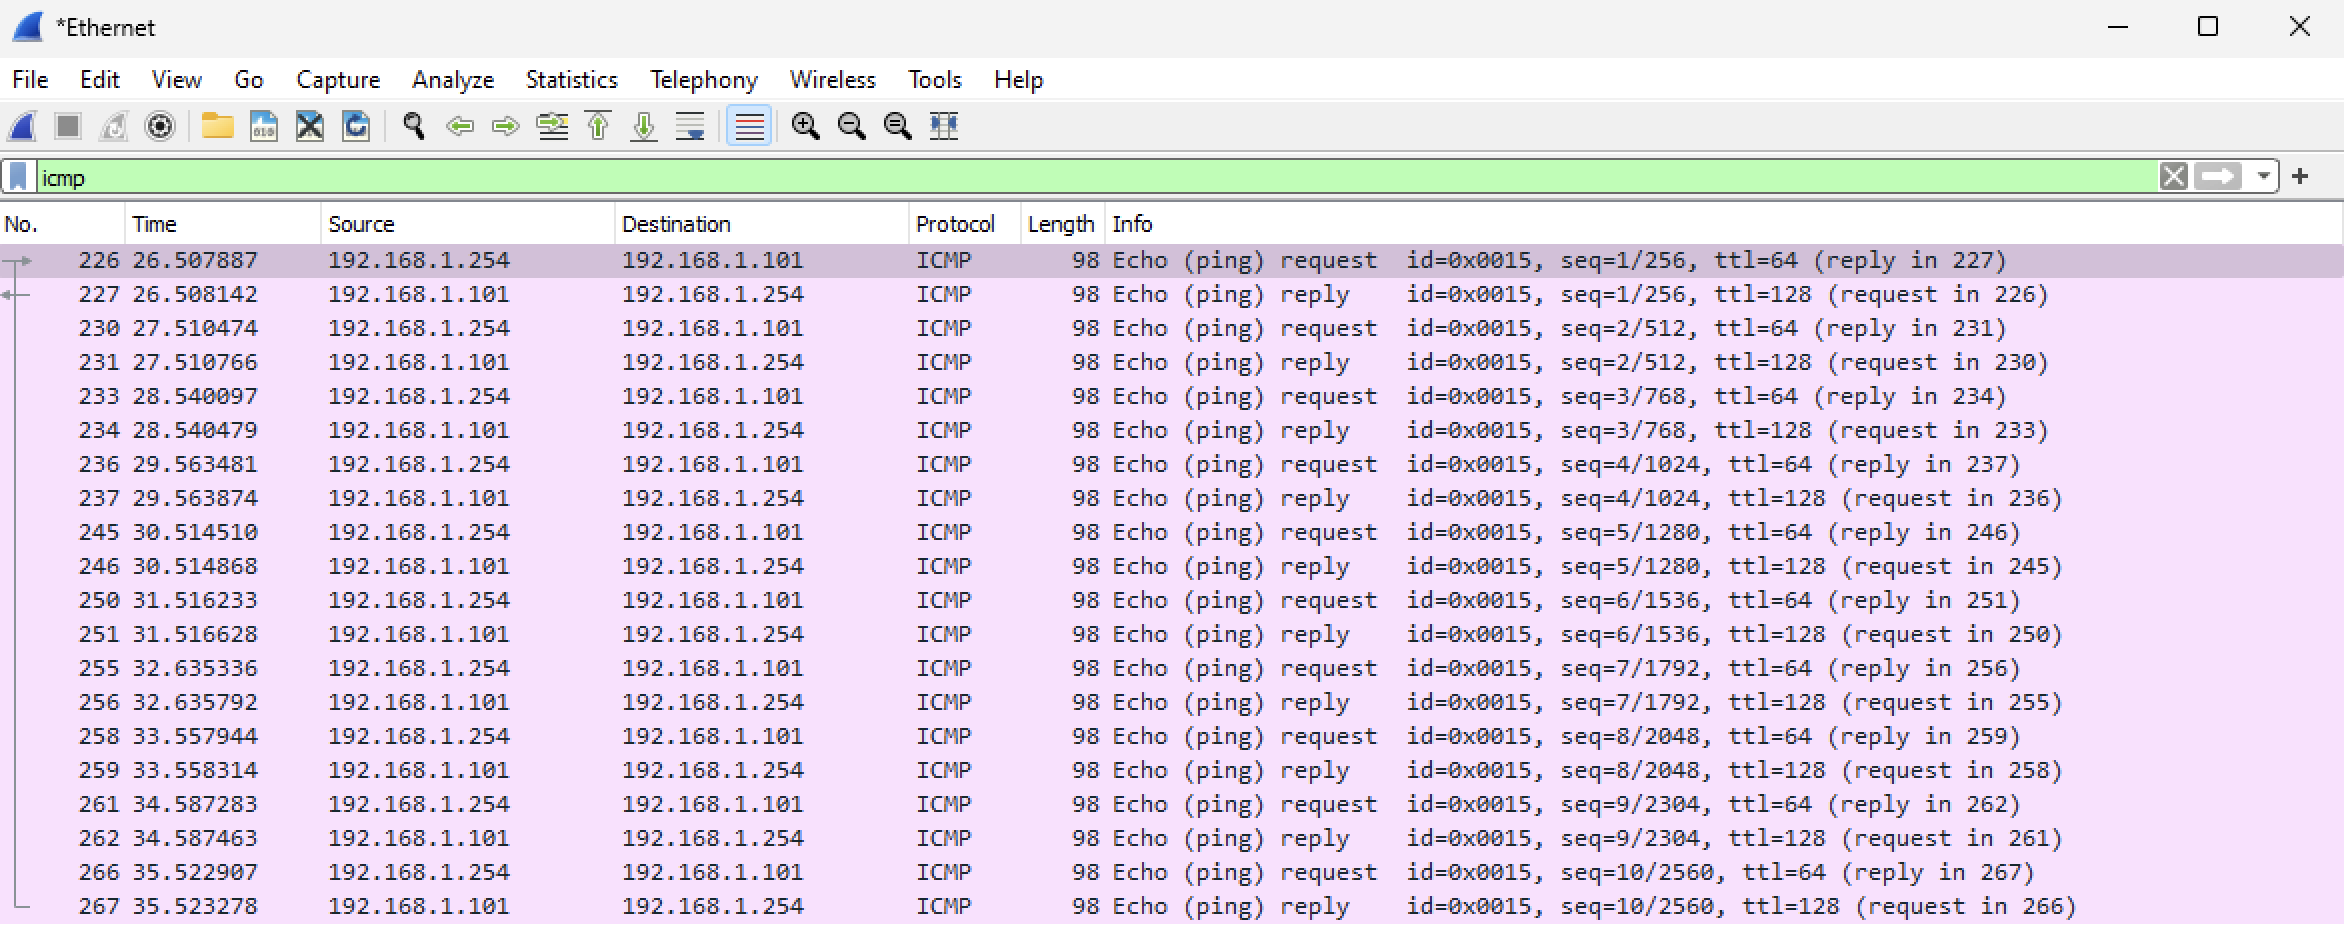
\includegraphics[width=0.85\textwidth]{images/icmp-result.png}
  \caption{Перехваченные ICMP-пакеты}
  \label{fig:icmp-result}
\end{figure}

Убедимся, что MAC-адреса отправителя и получателя совпадают с адресами на
компьютерах. Так как запрос осуществлялся с компьютера на операционной системе
Linux, воспользуемся утилитой ifconfig для получения MAC-адреса (рис.
\ref{fig:ifconfig}). Для получения MAC-адреса на компьютере получателя получим с
помощью утилиты ipconfig, так как лабораторная работа выполняется на
операционной системе Windows (рис. \ref{fig:ipconfig}).

\begin{figure}[H]
  \centering
  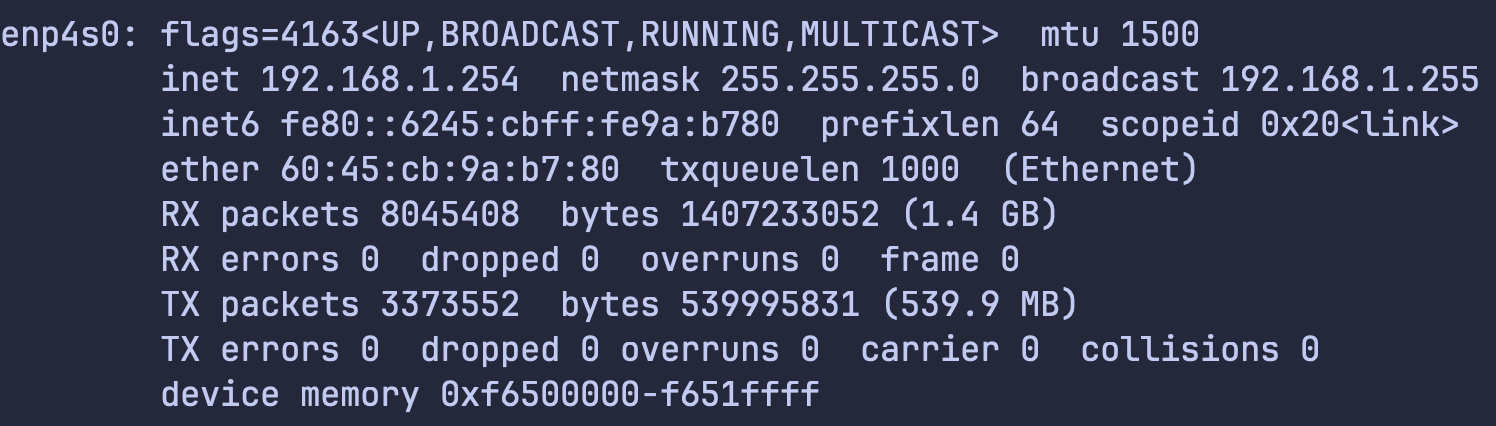
\includegraphics[width=0.8\textwidth]{images/ifconfig.png}
  \caption{Информация о MAC-адресе отправителя}
  \label{fig:ifconfig}
\end{figure}

\begin{figure}[H]
  \centering
  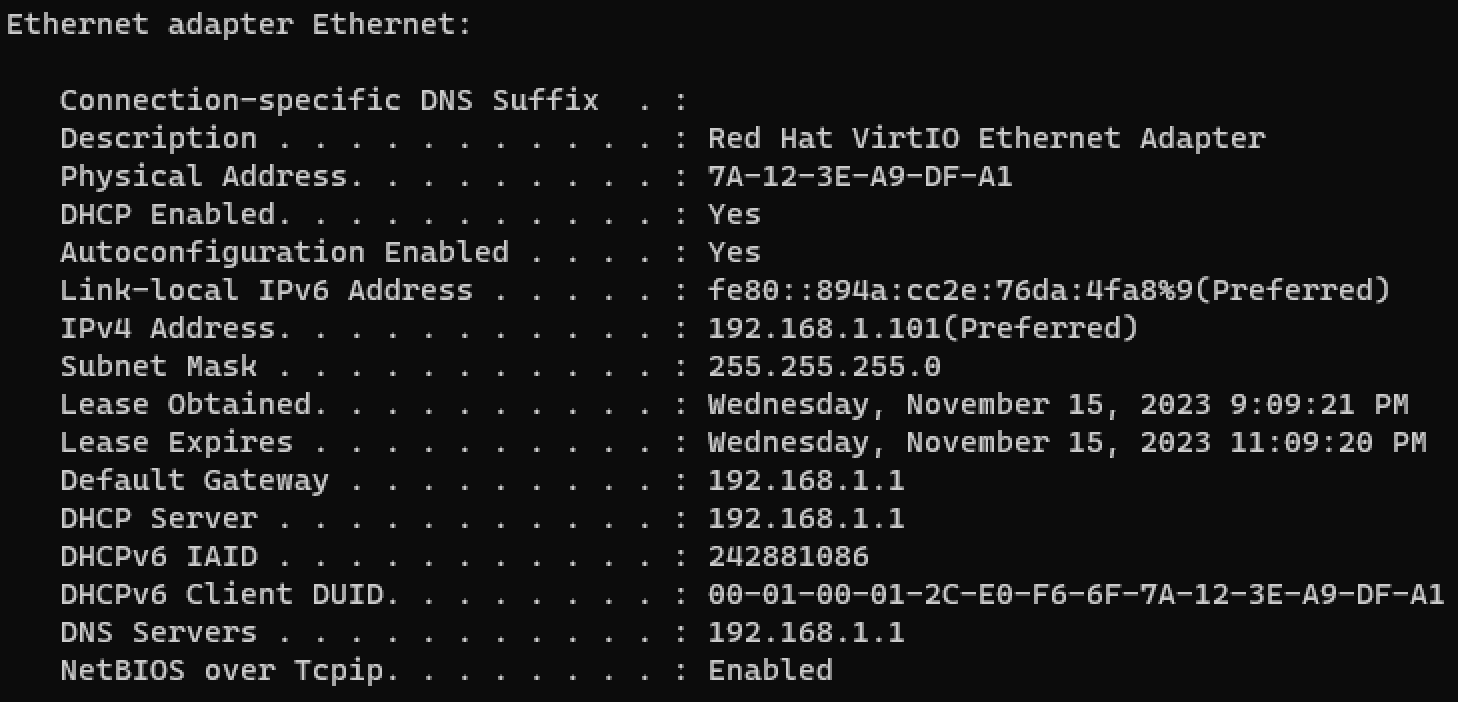
\includegraphics[width=0.8\textwidth]{images/ipconfig.png}
  \caption{Информация о MAC-адресе получателя}
  \label{fig:ipconfig}
\end{figure}

Теперь проверим содержимое полученных пакетов. Откроем вкладку <<Ethernet II>>
(рис. \ref{fig:ethernet-info}). Как видно, адреса совпадают с теми, что были
получены ранее. Несмотря на то, что ICMP-запрос выполнялся по IP адресу,
компьютеры смогли определить MAC-адреса друг друга. Это произошло с помощью
протокола ARP, который позволяет устройствам узнать MAC-адрес получателя по
IP-адресу.

\begin{figure}[H]
  \centering
  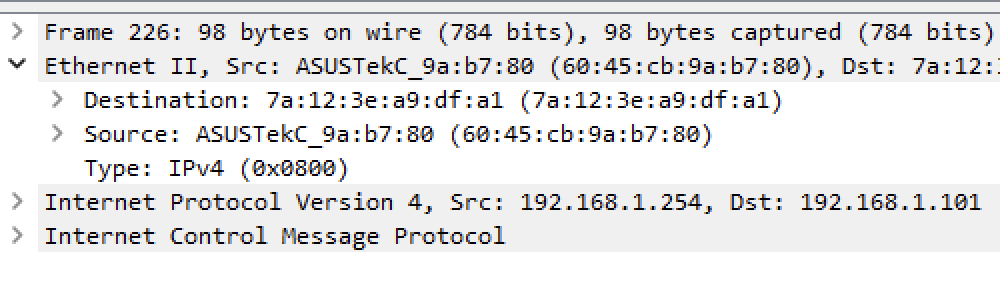
\includegraphics[width=0.8\textwidth]{images/ethernet-info.png}
  \caption{Информация о MAC-адресах в ICMP-пакете}
  \label{fig:ethernet-info}
\end{figure}

В качестве удаленных узлов (сайтов зарубежных СМИ) выберем следующие URL-адреса:
insider.com, theguardian.com и nytimes.com. Выполним ICMP-запросы с помощью
утилиты ping с включенным перехватом пакетов в Wireshark (рис.
\ref{fig:ping-remote}).

\begin{figure}[H]
  \centering
  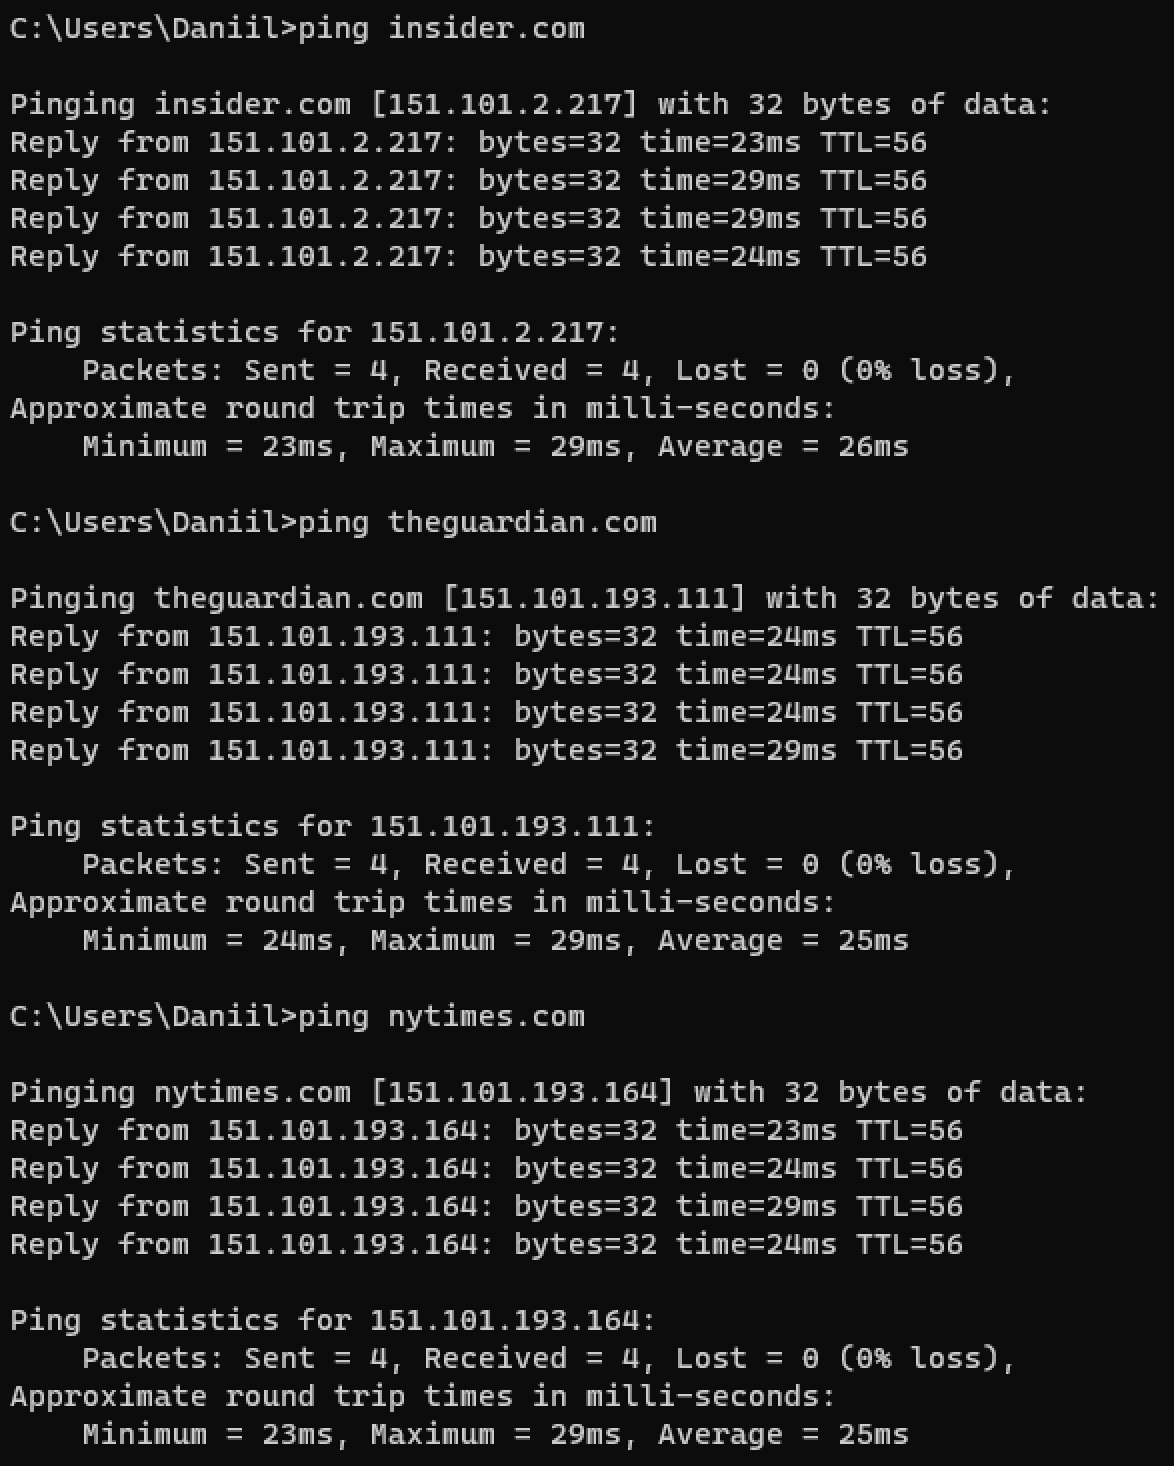
\includegraphics[width=0.65\textwidth]{images/ping-remote.png}
  \caption{ICMP-запросы на удаленные узлы}
  \label{fig:ping-remote}
\end{figure}

Как видно на рис. \ref{fig:ping-remote}, удаленные узлы имеют следующие
IP-адреса:
\begin{itemize}
  \item \textbf{insider.com}: 151.101.2.217;
  \item \textbf{theguardian.com}: 151.101.193.111;
  \item \textbf{nytimes.com}: 151.101.193.164.
\end{itemize}
Проанализируем пакеты в Wireshark. Как видно на рис.
\ref{fig:icmp-remote-1}-\ref{fig:icmp-remote-3}, IP-адреса отправителя и
получателя ICMP-запросов соответствуют ожидаемым. 

\begin{figure}[H]
  \centering
  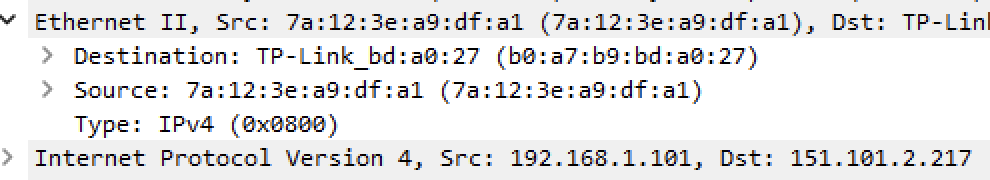
\includegraphics[width=0.8\textwidth]{images/icmp-remote-1.png}
  \caption{Информация о ICMP-запросе на первый удаленный узел}
  \label{fig:icmp-remote-1}
\end{figure}

\begin{figure}[H]
  \centering
  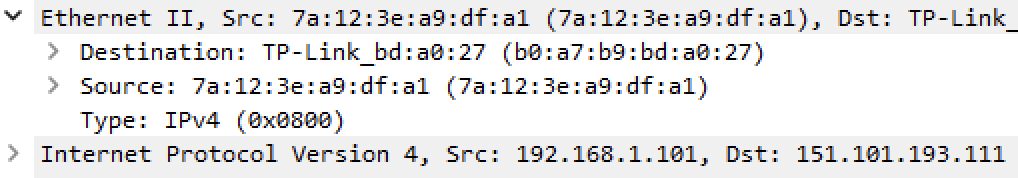
\includegraphics[width=0.8\textwidth]{images/icmp-remote-2.png}
  \caption{Информация о ICMP-запросе на второй удаленный узел}
  \label{fig:icmp-remote-2}
\end{figure}

\begin{figure}[H]
  \centering
  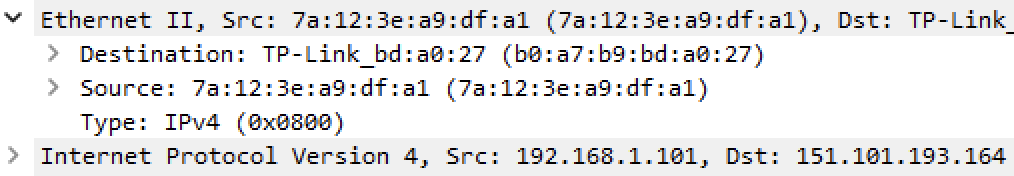
\includegraphics[width=0.8\textwidth]{images/icmp-remote-3.png}
  \caption{Информация о ICMP-запросе на третий удаленный узел}
  \label{fig:icmp-remote-3}
\end{figure}

Заметим, что MAC-адрес получателя всегда остается одним и тем же, несмотря на
изменение адреса удаленного узла. Это происходит потому, что все отправляемые
пакеты проходят через маршрутизатор, поскольку удаленные узлы находятся за
пределами локальной сети. Поэтому все MAC-адреса получателя совпадают с
MAC-адресом маршрутизатора (рис. \ref{fig:router-mac}).

\begin{figure}[H]
  \centering
  \fbox{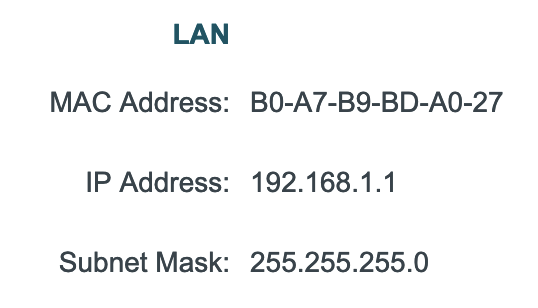
\includegraphics[width=0.5\textwidth]{images/router-mac.png}}
  \caption{Информация о MAC-адресе маршрутизатора}
  \label{fig:router-mac}
\end{figure}

\subsection{Анализ полей TCP}

В качестве FTP-сервера, к которому будет произведено подключение, был выбран
FTP-сервер Яндекса с адресом ftp.yandex.ru. Для того, чтобы лишние TCP-пакеты не
попадали при перехвате пакетов в Wireshark, необходимо было указать адрес
FTP-сервера. Для того, чтобы узнать адрес, использовалась утилита nslookup (рис.
\ref{fig:nslookup}).

\begin{figure}[H]
  \centering
  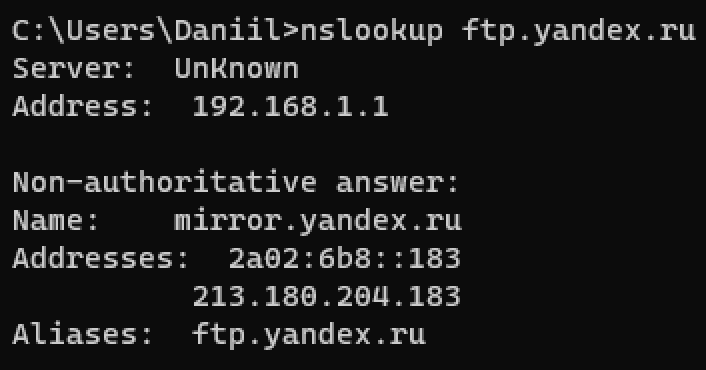
\includegraphics[width=0.7\textwidth]{images/nslookup.png}
  \caption{Нахождение IP-адреса FTP-сервера с помощью утилиты nslookup}
  \label{fig:nslookup}
\end{figure}

Для фильтрации перехватываемых пакетов использовался следующий фильтр:
\begin{minted}{text}
  tcp and ip.addr == 213.180.204.183
\end{minted}
В итоге были перехвачены пакеты, представленные на рис. \ref{fig:tcp-result}.

\begin{figure}[H]
  \centering
  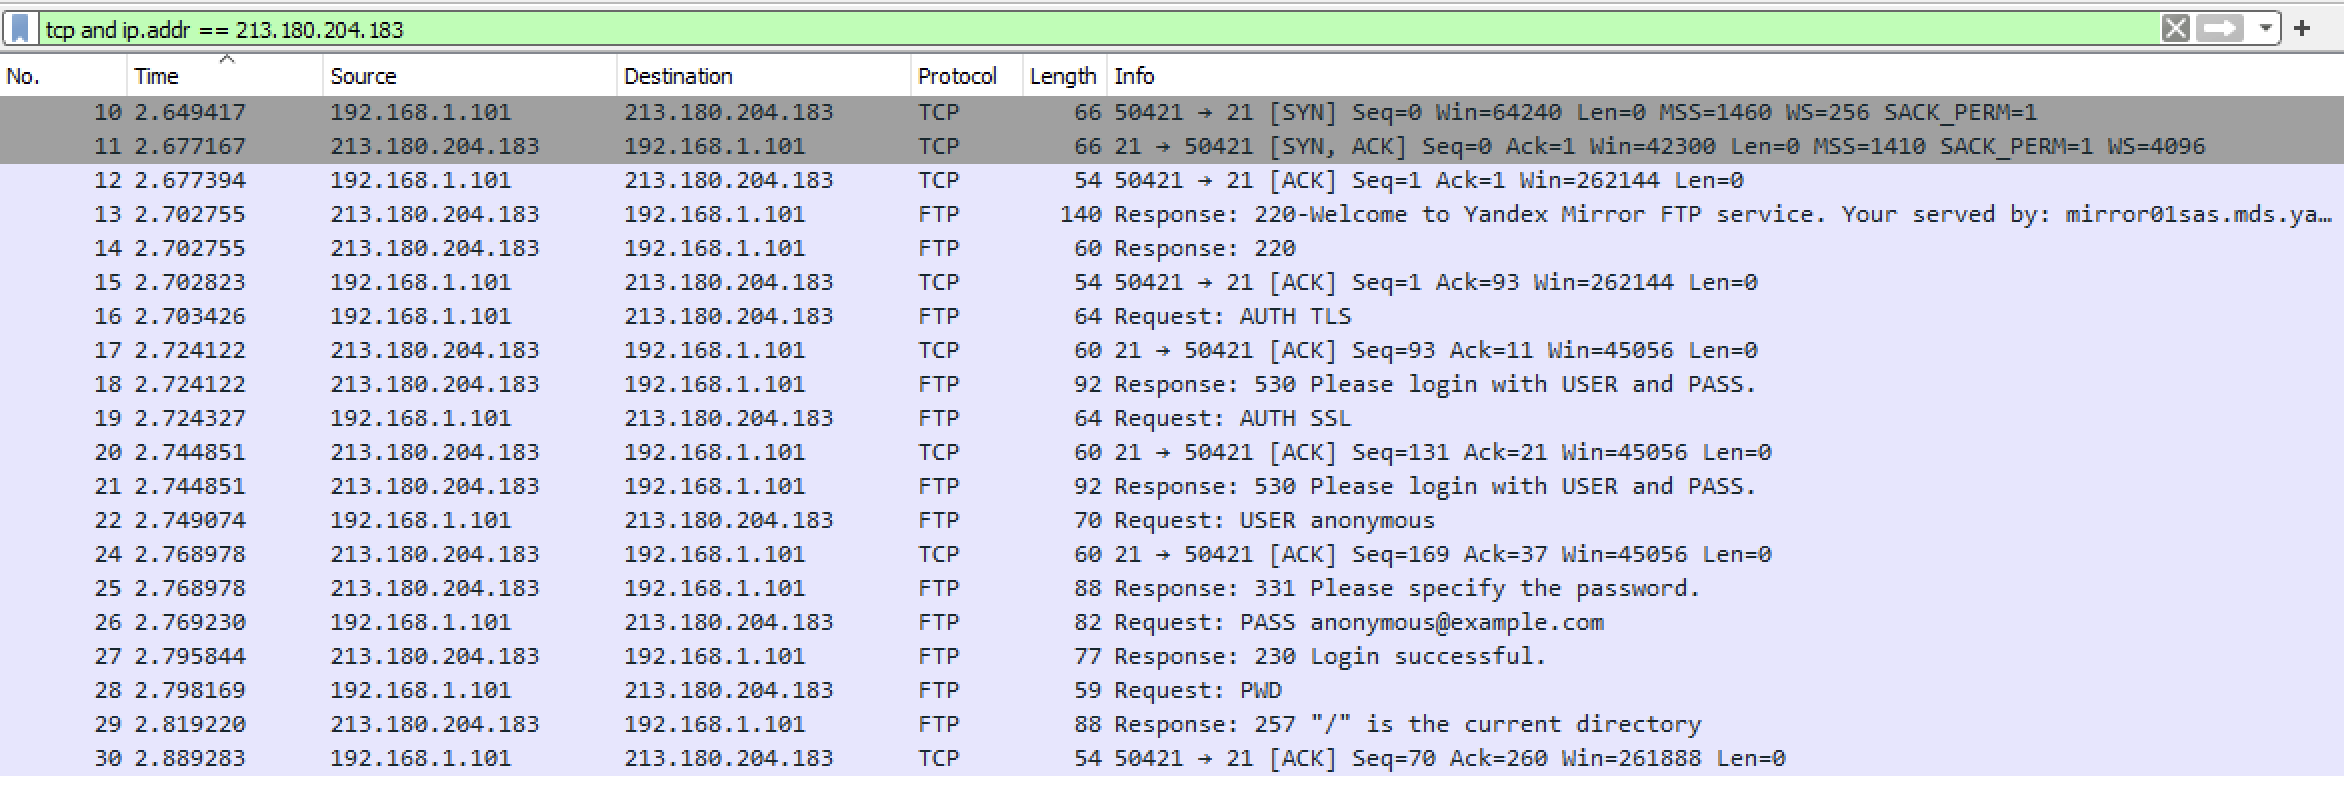
\includegraphics[width=\textwidth]{images/tcp-result.png}
  \caption{Перехваченные пакеты при подключении к FTP-серверу}
  \label{fig:tcp-result}
\end{figure}

Рассмотрим TCP-пакеты поочередно. Первый перехваченный TCP-пакет (рис.
\ref{fig:tcp-1}), имеет поля, которые находятся в таблице \ref{tab:tcp-1}.

\begin{figure}[H]
  \centering
  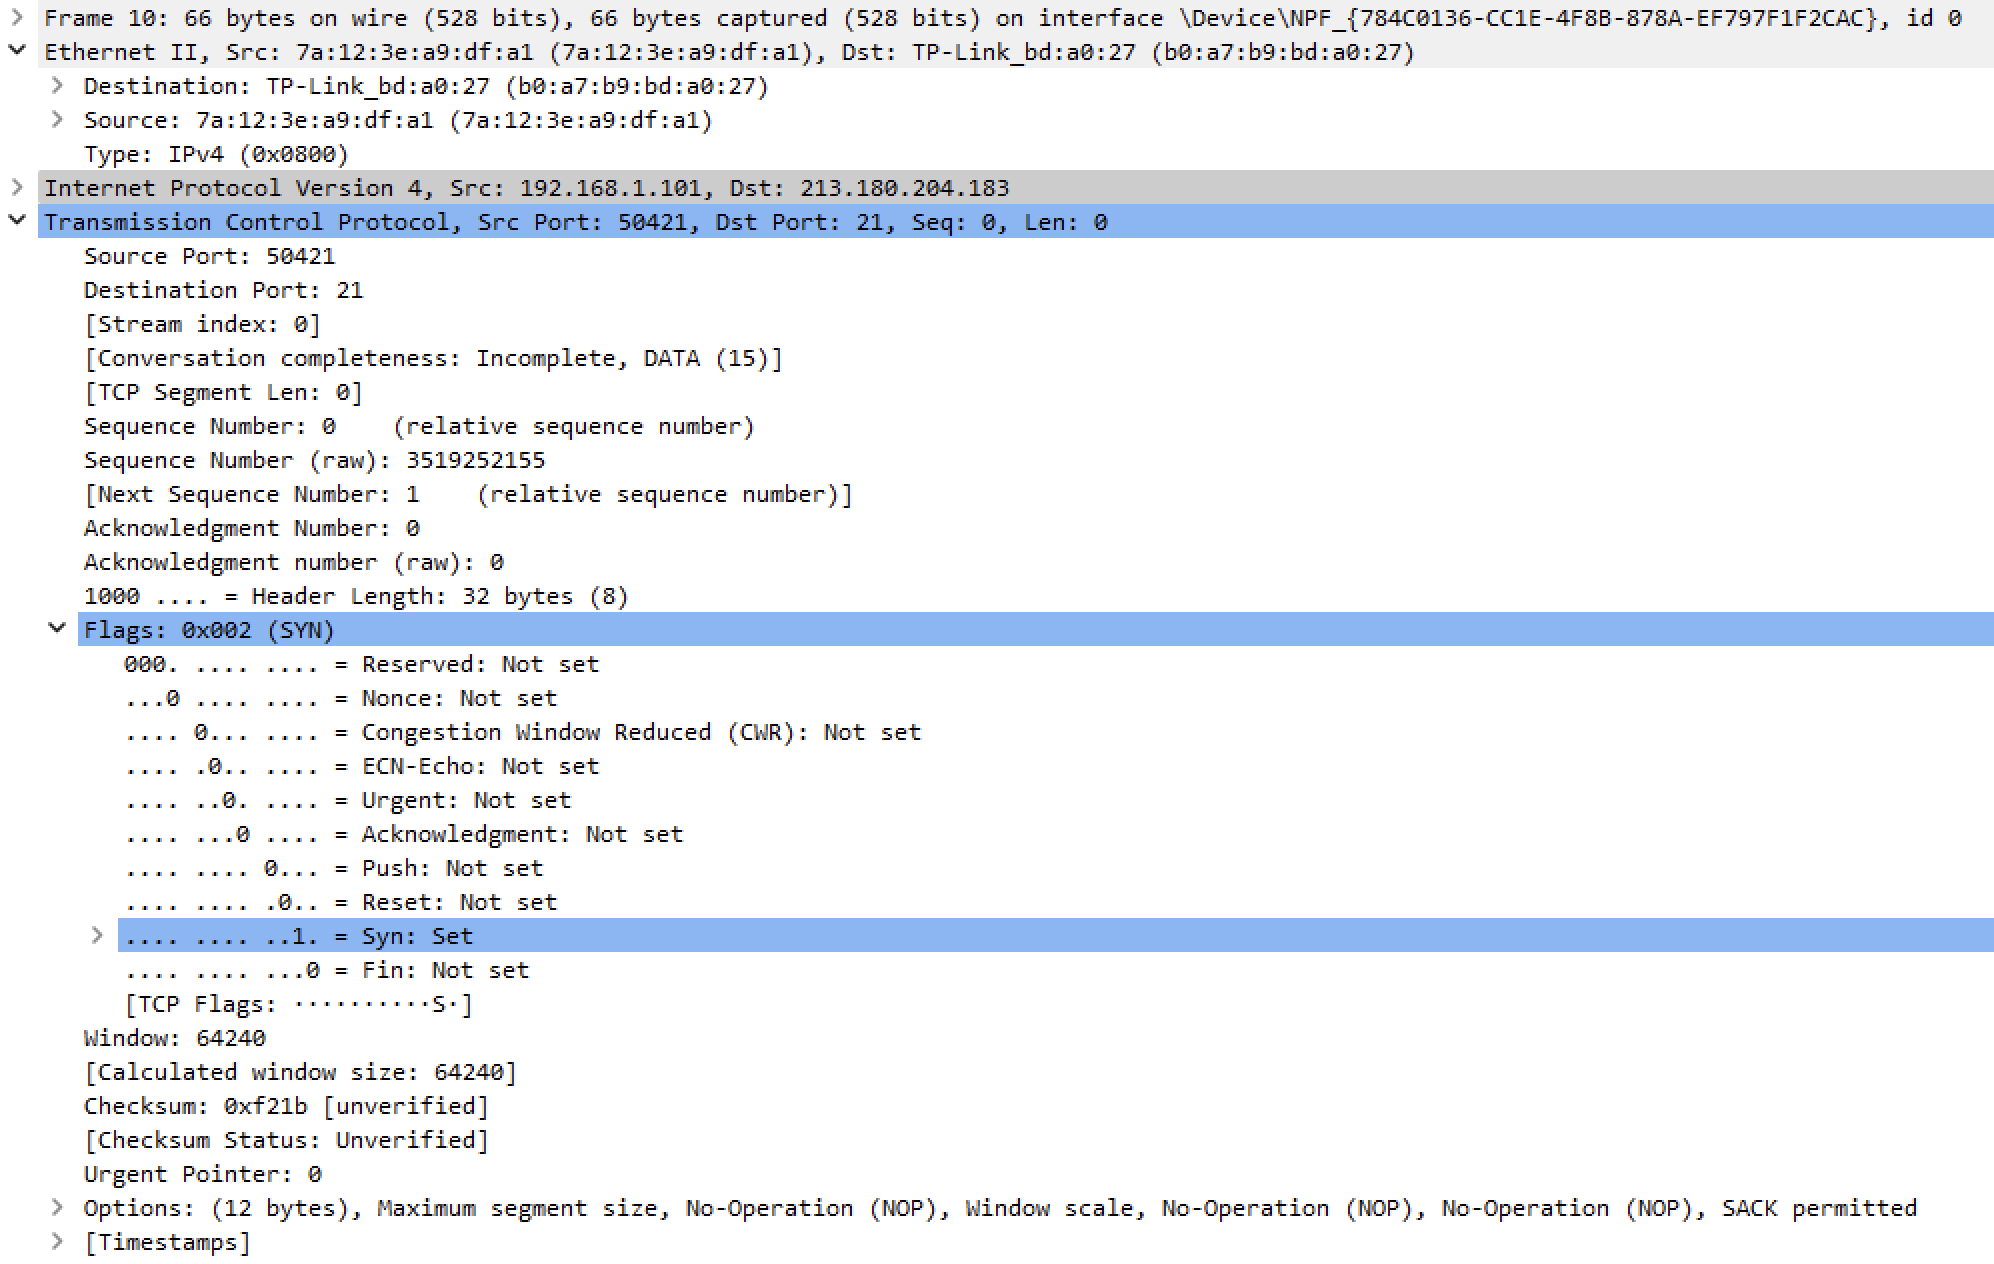
\includegraphics[width=\textwidth]{images/tcp-1.png}
  \caption{Первый перехваченный TCP-пакет}
  \label{fig:tcp-1}
\end{figure}

\begin{table}[H]
  \caption{Поля первого TCP-пакета}
  \label{tab:tcp-1}

  \centering
  \renewcommand*{\arraystretch}{1.2}
  \setlength{\tabcolsep}{12pt}

  \begin{tabular}{|c|c|}
    \hline
    \textbf{Название поля} & \textbf{Значение поля} \\
    \hline
    IP-адрес источника & 192.168.1.101 \\
    \hline
    IP-адрес назначения & 213.180.204.183 \\
    \hline
    Номер порта источника & 50421 \\
    \hline
    Номер порта назначения & 21 \\
    \hline
    Порядковый номер & 0 \\
    \hline
    Номер подтверждения & 0 \\
    \hline
    Длина заголовка & 32 \\
    \hline
    Размер окна & 64240 \\
    \hline
  \end{tabular}
\end{table}

Поля второго TCP-пакета (рис. \ref{fig:tcp-2}) находятся в таблице
\ref{tab:tcp-2}.

\begin{figure}[H]
  \centering
  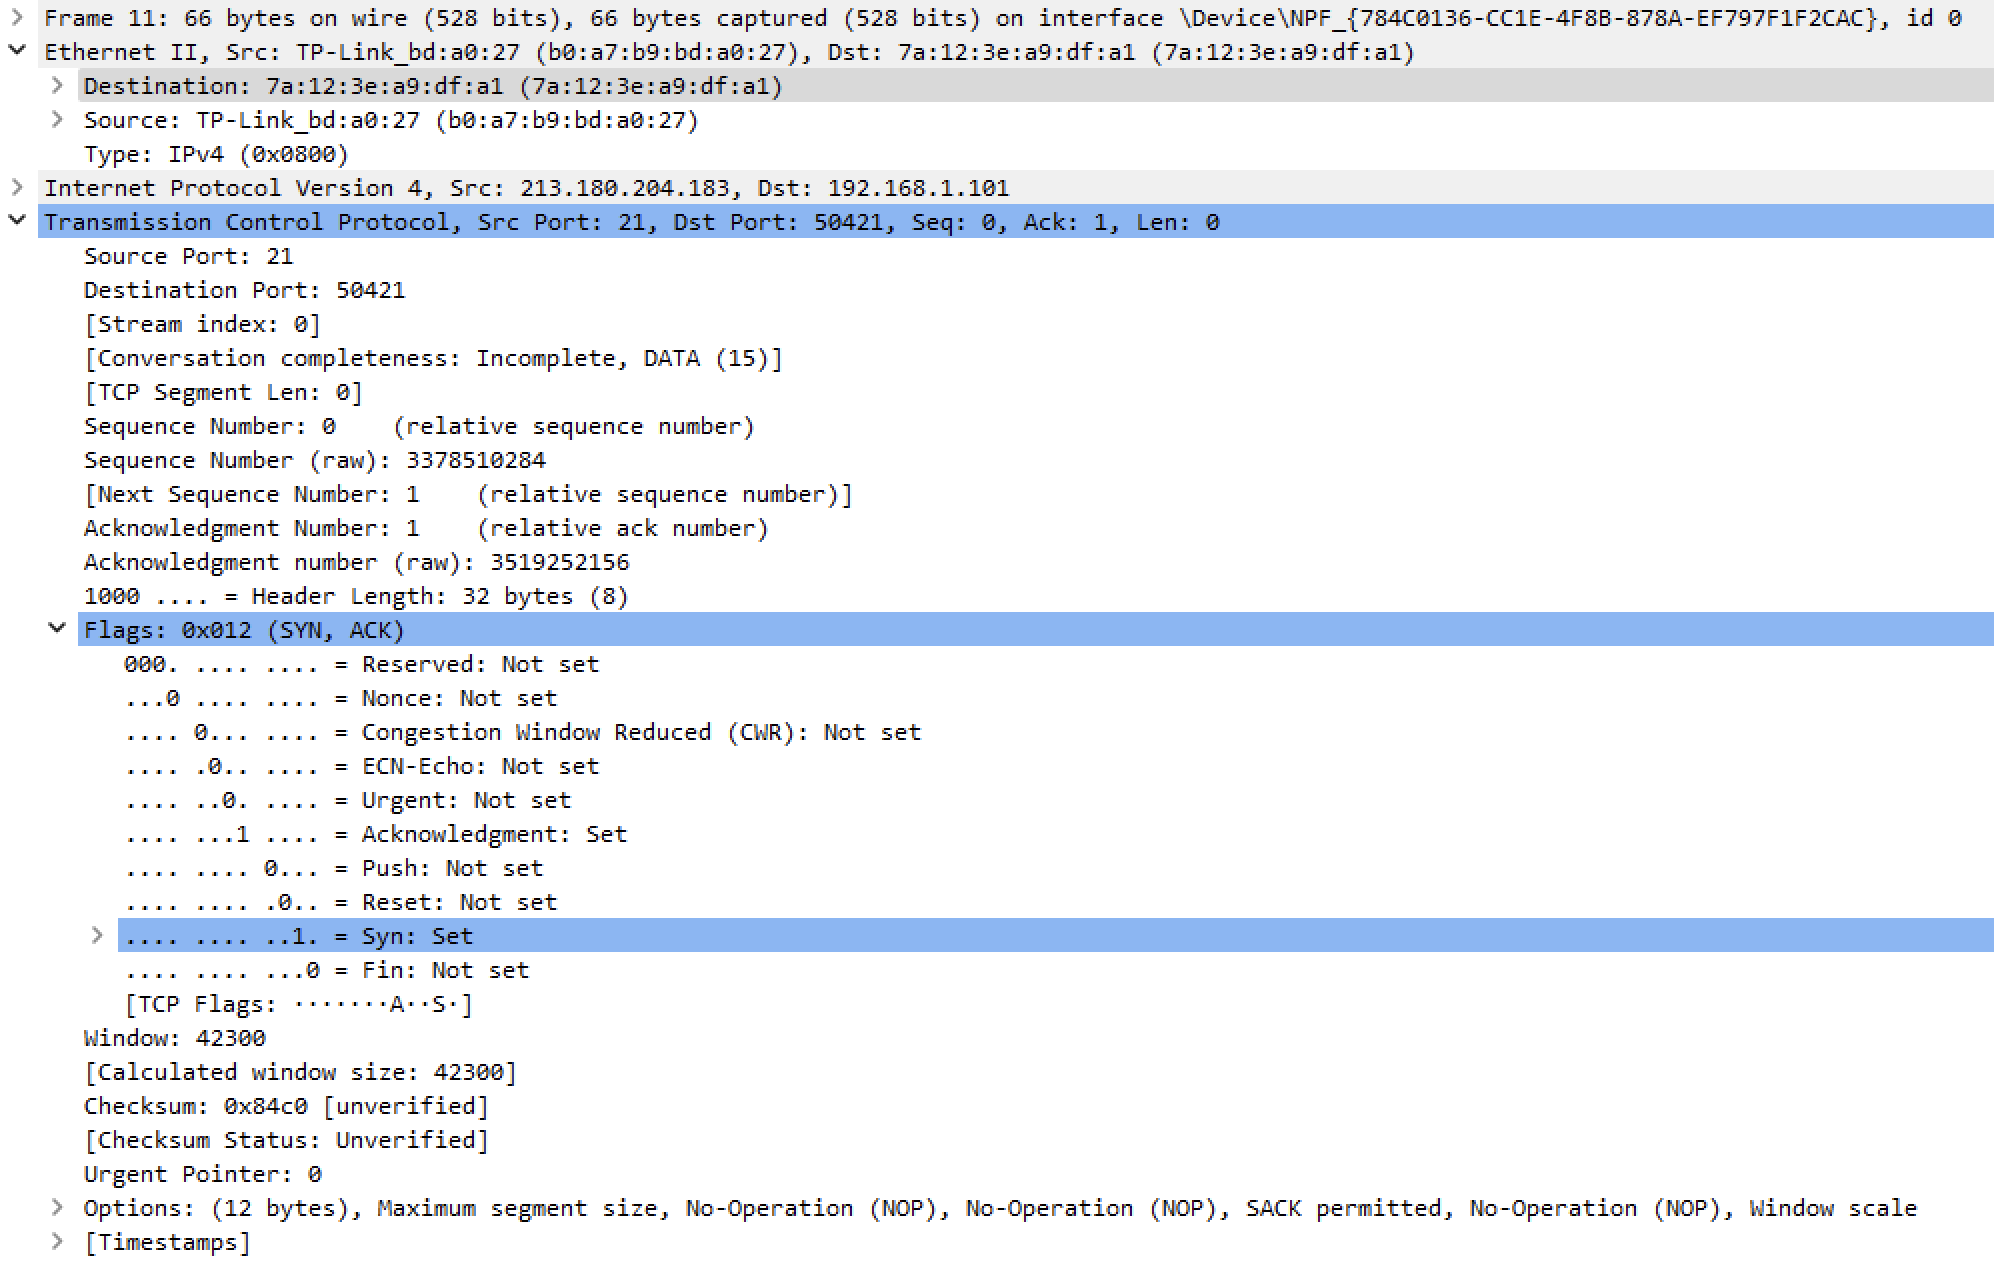
\includegraphics[width=\textwidth]{images/tcp-2.png}
  \caption{Второй перехваченный TCP-пакет}
  \label{fig:tcp-2}
\end{figure}

\begin{table}[H]
  \caption{Поля второго TCP-пакета}
  \label{tab:tcp-2}

  \centering
  \renewcommand*{\arraystretch}{1.2}
  \setlength{\tabcolsep}{12pt}

  \begin{tabular}{|c|c|}
    \hline
    \textbf{Название поля} & \textbf{Значение поля} \\
    \hline
    IP-адрес источника & 213.180.204.183 \\
    \hline
    IP-адрес назначения & 192.168.1.101 \\
    \hline
    Номер порта источника & 21 \\
    \hline
    Номер порта назначения & 50421 \\
    \hline
    Порядковый номер & 0 \\
    \hline
    Номер подтверждения & 1 \\
    \hline
    Длина заголовка & 32 \\
    \hline
    Размер окна & 42300 \\
    \hline
  \end{tabular}
\end{table}

Поля третьего TCP-пакета (рис. \ref{fig:tcp-3}) находятся в таблице
\ref{tab:tcp-3}.

\begin{figure}[H]
  \centering
  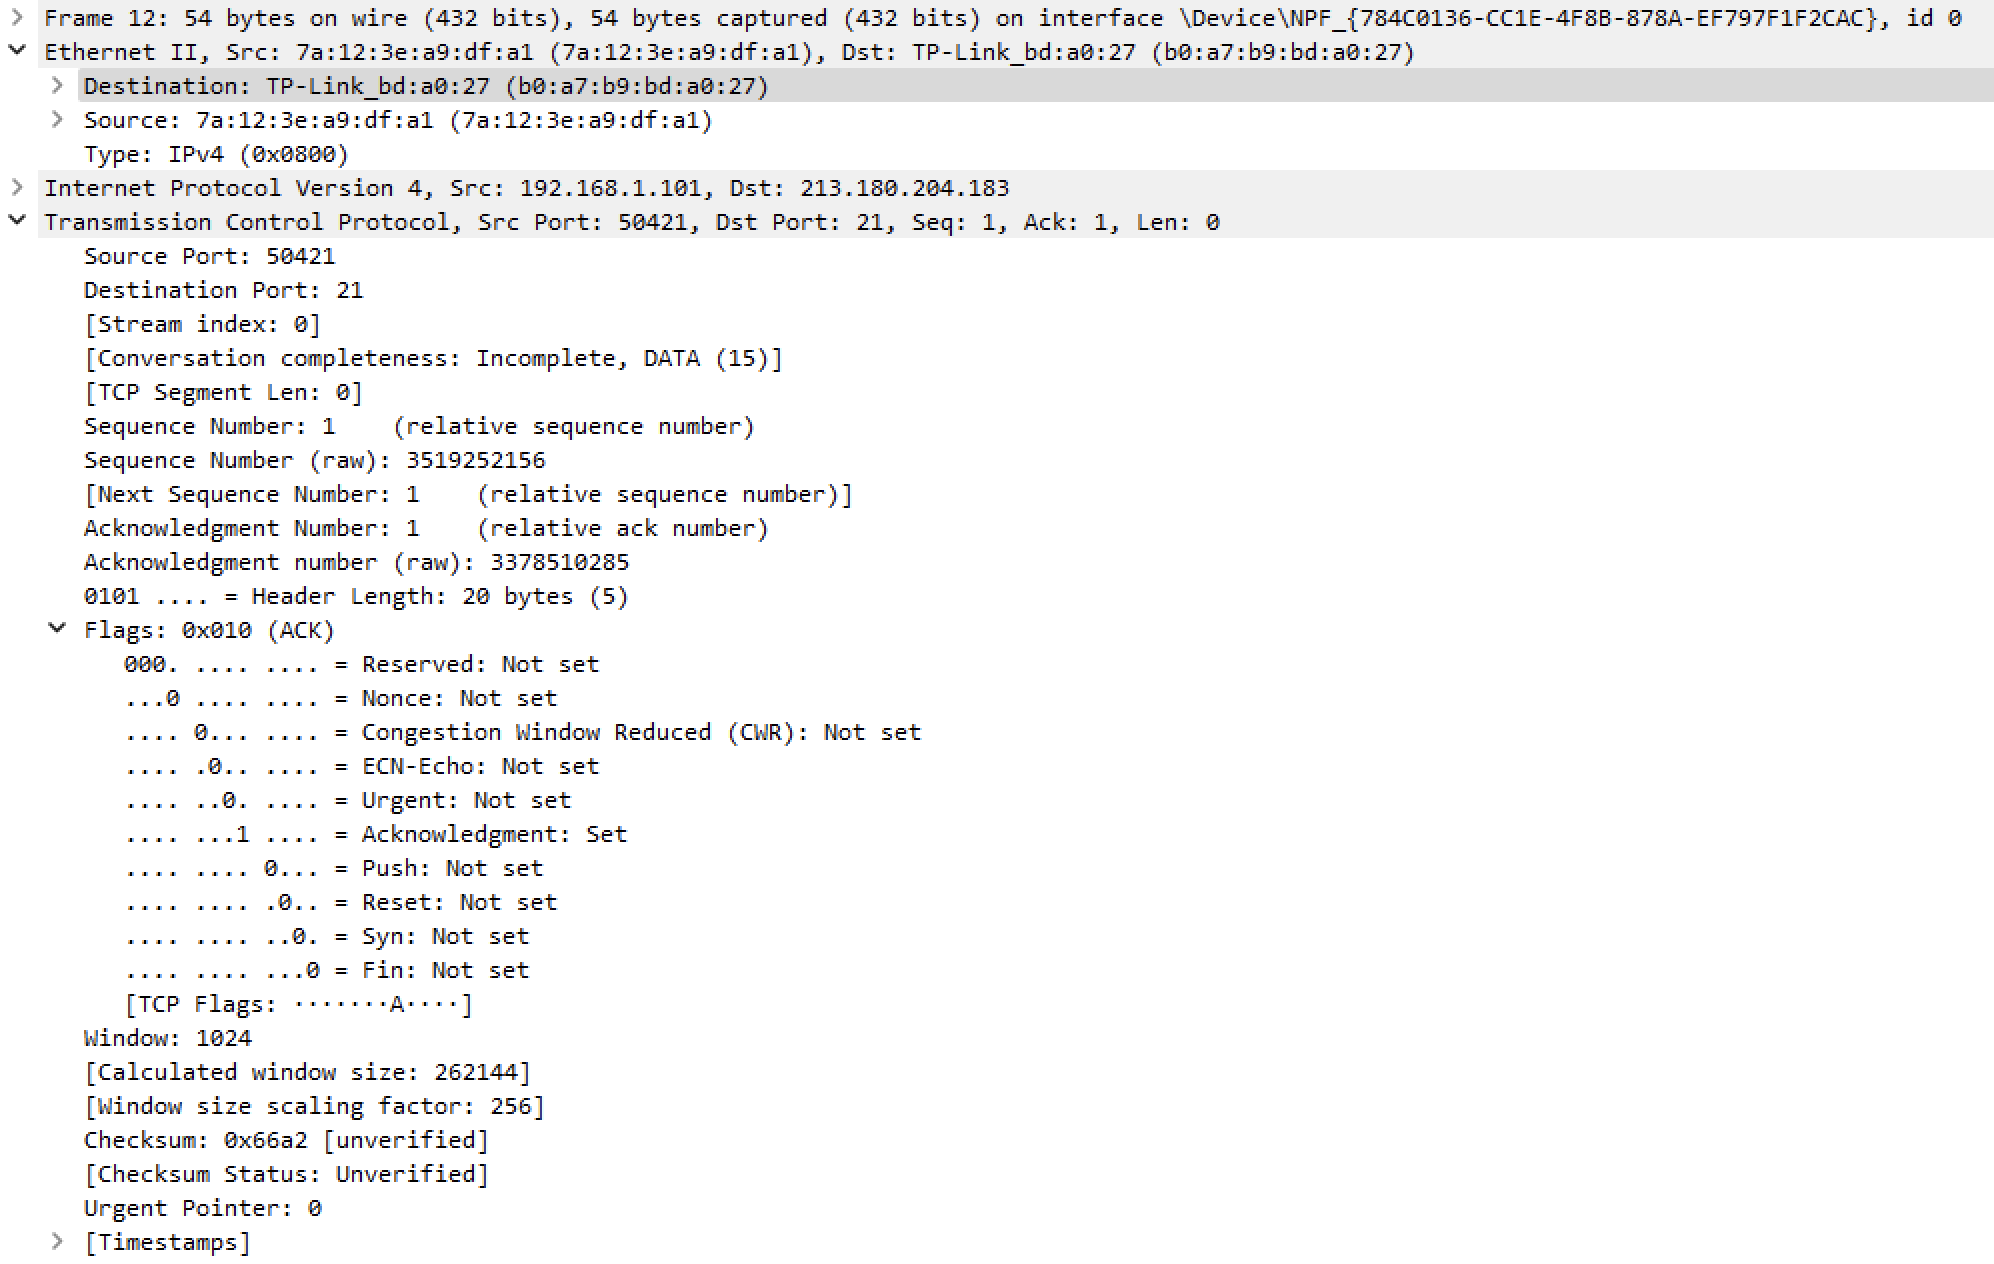
\includegraphics[width=\textwidth]{images/tcp-3.png}
  \caption{Третий перехваченный TCP-пакет}
  \label{fig:tcp-3}
\end{figure}

\begin{table}[H]
  \caption{Поля третьего TCP-пакета}
  \label{tab:tcp-3}

  \centering
  \renewcommand*{\arraystretch}{1.2}
  \setlength{\tabcolsep}{12pt}

  \begin{tabular}{|c|c|}
    \hline
    \textbf{Название поля} & \textbf{Значение поля} \\
    \hline
    IP-адрес источника & 192.168.1.101 \\
    \hline
    IP-адрес назначения & 213.180.204.183 \\
    \hline
    Номер порта источника & 50421 \\
    \hline
    Номер порта назначения & 21 \\
    \hline
    Порядковый номер & 1 \\
    \hline
    Номер подтверждения & 1 \\
    \hline
    Длина заголовка & 20 \\
    \hline
    Размер окна & 1024 \\
    \hline
  \end{tabular}
\end{table}

С помощью следующего фильтра
\begin{minted}{text}
  ftp and ip.addr == 213.180.204.183
\end{minted}
можно получить только те пакеты, что относятся к протоколу FTP (рис.
\ref{fig:ftp}).

\begin{figure}[H]
  \centering
  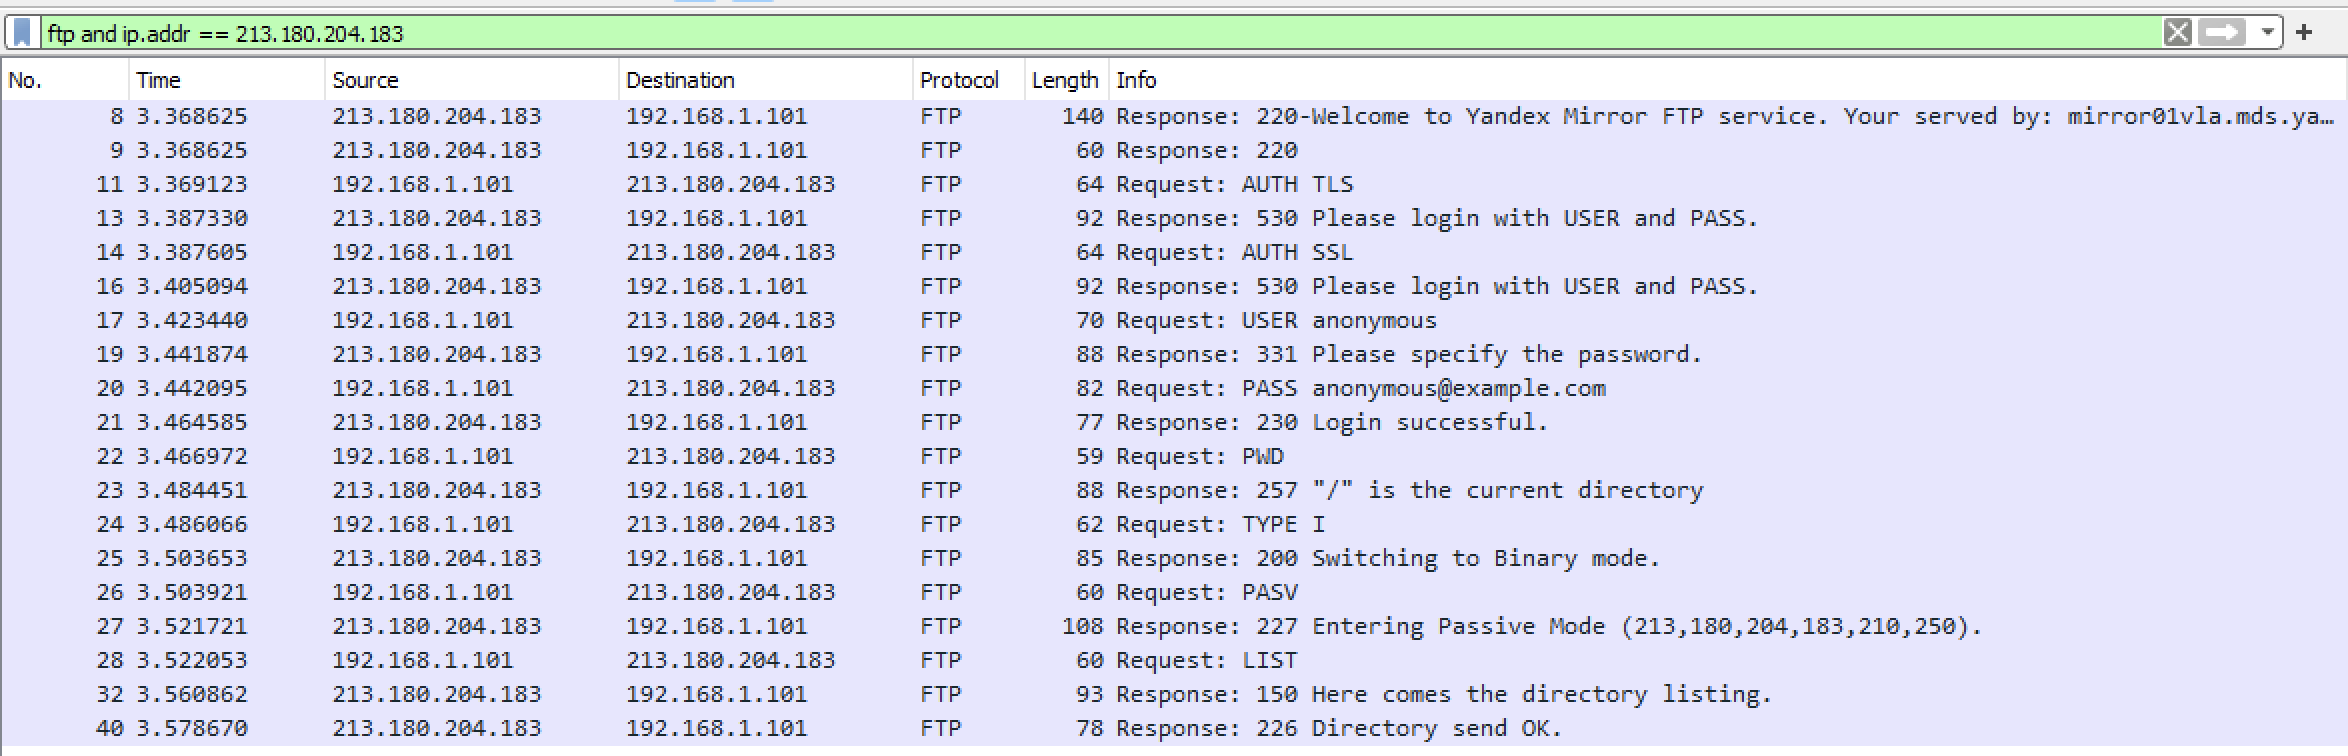
\includegraphics[width=\textwidth]{images/ftp.png}
  \caption{Перехваченные FTP-пакеты}
  \label{fig:ftp}
\end{figure}

\section{Заключение}

В ходе выполнения данной лабораторной работы я разобрался со стеком TCP/IP,
анализируя пакеты, которые отправляются и принимаются с помощью данного стека,
научился собирать сетевой трафик с помощью программы Wireshark, научился
фильтровать собранный трафик, находить и просматривать соединения.

\end{document}
